% =====================================================================
%  Main text. REVTeX 4.2, two-column.
%  For PRX Quantum submission replace "pra" by "prxquantum" in the class
%  options (requires a REVTeX build that ships the prxquantum option).
%  Compile order:  pdflatex supplement; pdflatex main (x3)
%  (main.tex reads supplement.aux through xr-hyper for "Sec. S3" etc.)
% =====================================================================
\documentclass[aps,pra,twocolumn,superscriptaddress,reprint,nofootinbib,floatfix]{revtex4-2}

\usepackage{amsmath,amssymb,amsthm,bm}
\usepackage{graphicx}
\usepackage{booktabs}
\usepackage{xcolor}
\usepackage[hidelinks,pdftitle={When does tail-risk optimization change a quantum gate?},
            pdfauthor={Sashreek Satapathy}]{hyperref}
\usepackage{xr-hyper}
\externaldocument[S-]{supplement}

\newtheorem{theorem}{Theorem}
\newtheorem{proposition}{Proposition}
\newtheorem{corollary}{Corollary}
\newtheorem{lemma}{Lemma}
\theoremstyle{definition}
\newtheorem{definition}{Definition}
\newtheorem{remark}{Remark}

\newcommand{\cvar}{\mathrm{CVaR}}
\newcommand{\E}{\mathbb{E}}
\newcommand{\Lt}{\widetilde L}
\newcommand{\Rt}{R_{\mathrm{tail}}}
\newcommand{\Rm}{R^{\mathrm{model}}}
\newcommand{\umean}{u_{\mathrm{mean}}}
\newcommand{\ucvar}{u_{\cvar}}
\newcommand{\SM}{Supplemental Material~\cite{SM}}
\newcommand{\sref}[1]{Sec.~\ref{S-#1}}

\graphicspath{{figures/}}
% panel label overlaid at the top-left corner of a graphic
\newcommand{\panel}[2]{\begingroup\setbox0\hbox{#2}%
  \leavevmode\rlap{\raisebox{\dimexpr\ht0-1.1em\relax}{\hspace{0.1em}\footnotesize(#1)}}\box0\endgroup}

\begin{document}

\title{When does tail-risk optimization change a quantum gate?\\
An equivalence boundary for mean and CVaR control}

\author{Sashreek Satapathy}

\date{\today}

\begin{abstract}
Robust quantum control usually minimizes the \emph{mean} gate error over
calibration noise, although fault tolerance is limited by rare bad gates.
Tail-risk objectives such as the conditional value-at-risk (CVaR) have been
proposed, but it is not known when they actually select a different pulse.
We prove that when the noise is Gaussian and enters the gate error linearly,
the error distributions of all controls are rescaled copies of one shape. All
controls are then ordered by stochastic dominance, and the mean, CVaR and
every other law-invariant monotone risk measure share one minimizer, up to an
explicit residual from the periodicity of the infidelity. The ordering
survives temporally correlated noise and several channels on one axis, and
fails for channels on different axes. Simulations of a transmon
$X_{\pi/2}$ gate, with full Lindblad re-evaluation, confirm the equivalence up
to an accumulated detuning phase variance of about 0.05 at three gate times.
Over pools of about 400 candidate pulses per setting, not one of 19\,639
well-separated pairs is ranked differently by the two objectives, and the
predicted tail-to-mean ratio of 5.58 holds to 2\%. Leakage does not break
the equivalence. Beyond the boundary, CVaR lowers the worst-5\% error by up to
37\% by deliberately miscalibrating the gate to pre-compensate the
second-order error of the worst noise draws. The ratio $\kappa$ of second- to
first-order error orders every divergence, and a parameter-free reduced model
bounds and ranks them in a prospective test. We show that the attainable gain
grows only as $\kappa^2$, derive its coefficient in closed form, and thereby
predict the threshold at which tail-risk optimization starts to pay. A
controlled experiment that holds $\kappa$ fixed while varying the gate time
and the noise correlation shows that this coefficient, not $\kappa$ alone, is
what explains the gain. Under Ornstein--Uhlenbeck noise the comparison is
unchanged across two decades of correlation time once that coefficient is held
fixed, as the theory requires. Colored noise instead changes the shape of the
tail, and we show that the tail-to-mean ratio measures the number of
independent noise directions reaching the gate: one law that contains both the
single-channel ratio 5.58 and the two-channel ratio 4.00, and that predicts
each control's ratio from its geometry to 3\%. Rotating the noise between two
channels raises that number by a mechanism with no time structure, and the
residuals from the two routes are statistically indistinguishable. Finally,
adding trajectory-level $T_1$ relaxation gives a rare catastrophic channel
whose effect on the tail-to-mean ratio we predict in closed form to 1\% across
a factor of 640 in its share of the mean loss --- and which nonetheless leaves
the selected pulse unchanged, because the gate requirement pins the channel to
within a percent whatever the objective. Tail weight without control leverage
buys nothing, a condition that $\kappa$ does not see.
\end{abstract}

\maketitle

% =====================================================================
\section{Introduction}
\label{sec:intro}

Quantum gates are calibrated against parameters that drift: the qubit
frequency wanders with two-level fluctuators and flux noise, and the drive
amplitude with the electronics \cite{Paladino2014,Krantz2019,Kjaergaard2020}.
Robust optimal control designs pulses that tolerate such drifts, usually by
maximizing the fidelity averaged over an ensemble of noise realizations
\cite{Khaneja2005,Glaser2015,Chen2014,Kosut2013,Weidner2025} or by cancelling
the leading orders of the error analytically or through filter functions
\cite{Wimperis1994,Green2013,Poggi2024,Ball2021}. The mean is a natural
target, but it is not the quantity a fault-tolerant processor is most
sensitive to. A surface-code threshold is a bound on the error of every
gate in every round \cite{Fowler2012}; a gate that is excellent on average
and poor on the few days the drift is large may be worse, in practice, than
one that is slightly worse on average and never poor.

Risk measures from finance make this concern quantitative. The conditional
value-at-risk,
\begin{equation}
\cvar_\alpha(X)=\min_{\tau\in\mathbb R}\Big\{\tau+\tfrac1\alpha\,\E\big[(X-\tau)_+\big]\Big\},
\label{eq:ru}
\end{equation}
is the mean of the worst $\alpha$ fraction of outcomes
\cite{Rockafellar2000,Acerbi2002}; it is coherent \cite{Artzner1999}, convex
in the decision variables and straightforward to optimize by sampling. CVaR
has been adopted as the objective of variational quantum optimization
\cite{Barkoutsos2020} and of quantum risk analysis \cite{Woerner2019}, and
risk-sensitive objectives based on exponential utility have been proposed
for robust quantum gates \cite{Ge2021}, where they were observed to select
controls different from those of the average fidelity. What has not been
established is \emph{when} a tail objective changes the answer. If the mean-
and tail-optimal controls coincide, CVaR adds only estimation noise, since it
is computed from a small fraction of the samples. If they differ, one needs
to know by how much and for what physical reason.

In portfolio theory the analogous question has a classic answer: for normal
or, more generally, elliptically distributed returns, every positively
homogeneous translation-invariant risk measure produces the same efficient
portfolios as the variance
\cite{Rockafellar2000,Embrechts2002}. The quantum problem differs in two
ways. The loss is a periodic, bounded function of the error, not a linear
one, and the noise can enter through several non-commuting generators and
beyond linear order.

In this paper we give a sharp answer for single-qubit gates under
quasi-static noise and test it at scale. Our contributions are:
\begin{enumerate}
\item A theorem (Sec.~\ref{sec:theory}) stating that if the noise is Gaussian
and couples linearly, every control's infidelity is a function of a single
scalar, so the loss family is totally ordered by first-order stochastic
dominance and all law-invariant monotone risk measures, including CVaR and
exponential utility, share the mean-optimal control. The periodicity of
$\sin^2(\phi/2)$ is handled by a monotone majorant with an explicit residual.
\item A characterization of how the ordering fails: two channels on
non-parallel axes break it through a Schur-convexity effect, and second-order
error does so through a pre-compensation mechanism, quantified by the ratio
$\kappa$ of second- to first-order error and by a parameter-free reduced
model. The tail gain is \emph{quadratically} small in $\kappa$, with a closed
form for its coefficient, which is why a sharp practical threshold exists at
all.
\item A numerical test on a four-level transmon with an audited protocol that
guards against optimization artefacts (Sec.~\ref{sec:model}). The equivalence
holds wherever the accumulated detuning phase variance satisfies
$\sigma_\phi^2\lesssim0.05$, at three gate times and including the regime in
which naive pulses leak strongly (Sec.~\ref{sec:equiv}); the dominance premise
itself holds over hundreds of candidate controls per setting
(Sec.~\ref{sec:dominance}).
\item An account of what CVaR does beyond the boundary: it deliberately
miscalibrates the nominal gate, with an offset that matches a parameter-free
prediction (Sec.~\ref{sec:mechanism}).
\end{enumerate}
The practical result (Sec.~\ref{sec:discussion}) is a test that can be run
on the mean-optimal control alone and says whether a tail objective can
help.

% =====================================================================
\section{Theory}
\label{sec:theory}

\subsection{Setup}

Consider a qubit whose control-frame Hamiltonian contains a classical noise
process $\eta(t)$ that couples linearly, so that the accumulated phase error
of a control $u$ with toggling-frame modulation function $f_u(t)$ is
\begin{equation}
\phi[u]=\int_0^{T_g}f_u(t)\,\eta(t)\,dt .
\label{eq:phase}
\end{equation}
The single-state infidelity of the resulting error rotation is
$L=h(\phi)=\sin^2(\phi/2)$; for a coherent rotation the average-gate
infidelity is $\tfrac23h(\phi)$ \cite{Nielsen2002}, so all statements below
hold for either figure of merit. We work under two hypotheses:
\textbf{(A1)} $\eta$ is a Gaussian process; \textbf{(A2)} $\phi[u]$ is
exactly the linear functional \eqref{eq:phase}. Then
$\phi[u]\sim\mathcal N(0,\sigma_u^2)$, and the whole loss distribution of a
control depends on the control only through the scalar $\sigma_u$. A control
cannot change the \emph{shape} of the phase distribution, only its width.

\subsection{Equivalence}

If $h$ were increasing in $|\phi|$, a narrower phase distribution would give
a loss that is smaller at every quantile, and the theorem would be immediate.
But $h$ is $2\pi$-periodic and decreases on $[\pi,2\pi]$, which is exactly
where CVaR looks. We therefore replace $h$ by its monotone majorant
$\Lt(\phi)=h(\phi)\mathbf 1(|\phi|\le\pi)+\mathbf 1(|\phi|>\pi)$
[Fig.~\ref{fig:theory}(a)] and bound the difference. Because
$\Lt-h\le\mathbf 1(|\phi|>\pi)$ and CVaR is monotone and subadditive, with
$\cvar_\alpha(\mathbf 1_E)=\min(1,\Pr E/\alpha)$, we obtain the sandwich
\begin{equation}
\cvar_\alpha\big(\Lt(\phi)\big)-r_\alpha(\sigma)\le\cvar_\alpha\big(h(\phi)\big)\le\cvar_\alpha\big(\Lt(\phi)\big),
\label{eq:sandwich}
\end{equation}
with residual
\begin{equation}
r_\alpha(\sigma)=\frac{\Pr(|\phi|>\pi)}{\alpha}\le\frac1\alpha\sqrt{\frac2\pi}\,\frac{\sigma}{\pi}\,e^{-\pi^2/2\sigma^2}.
\label{eq:residual}
\end{equation}

\begin{theorem}[Mean--CVaR near-equivalence]
\label{thm:main}
Under (A1)--(A2), let two controls have $\sigma_1<\sigma_2$ and let
$Z\sim\mathcal N(0,1)$. Then the mean loss
$\E h(\phi)=\tfrac12(1-e^{-\sigma^2/2})$ is strictly larger for the second,
and
\begin{equation*}
\cvar_\alpha\big(h(\phi_2)\big)-\cvar_\alpha\big(h(\phi_1)\big)\ge\Delta_{\mathrm{mono}}-r_\alpha(\sigma_2),
\end{equation*}
where $\Delta_{\mathrm{mono}}=\cvar_\alpha\big(\Lt(\sigma_2Z)\big)-\cvar_\alpha\big(\Lt(\sigma_1Z)\big)\ge0$.
Hence the two objectives order the controls identically whenever
$\Delta_{\mathrm{mono}}>r_\alpha(\sigma_2)$, and the mean-optimal control
is CVaR-optimal whenever this holds against every competitor.
\end{theorem}

\begin{proof}[Proof sketch]
$\sigma_2|Z|\ge\sigma_1|Z|$ pointwise and $\Lt$ is non-decreasing in
$|\phi|$, so $\Lt(\sigma_2Z)\ge\Lt(\sigma_1Z)$ pointwise and
$\Delta_{\mathrm{mono}}\ge0$ by monotonicity of CVaR. Apply the upper half of
Eq.~\eqref{eq:sandwich} to the first control and the lower half to the
second. The mean follows from $\E\cos\phi=e^{-\sigma^2/2}$, which integrates
over the periodicity exactly. Full proofs are in \sref{sec:proofs}.
\end{proof}

The residual is negligible at any noise level of interest: at $\alpha=0.05$
and $\sigma^2=0.05$ (mean infidelity 1.2\%), $r_\alpha\approx1.5\times10^{-43}$,
while $\Delta_{\mathrm{mono}}$ between meaningfully different controls is of
order $\sigma^2$. The theorem is a statement about the ranking of controls,
not about the value of the objectives. The values differ by a
control-independent factor:

\begin{proposition}[Tail amplification]
\label{prop:ratio}
As $\sigma^2\to0$, $\cvar_\alpha(h(\phi))/\E h(\phi)\to1+2z_\alpha\varphi(z_\alpha)/\alpha$,
with $z_\alpha=\Phi^{-1}(1-\alpha/2)$ and $\varphi$ the standard normal
density. The ratio is $3.25$, $4.39$, $5.58$, $6.80$ and $8.45$ at
$\alpha=0.2$, $0.1$, $0.05$, $0.025$ and $0.01$.
\end{proposition}

This follows from $h\approx\phi^2/4=\sigma^2Z^2/4$: the loss is a rescaled
$\chi^2_1$ variable, and the tail average of $Z^2$ over $|Z|>z_\alpha$ is
obtained by integration by parts. Proposition~\ref{prop:ratio} gives a
second, independent test of the theorem: in the equivalence regime
\emph{every} control must have the same tail-to-mean ratio.

The argument uses nothing specific to CVaR. It needs only that the family of
loss distributions be totally ordered:

\begin{corollary}[Dominance principle]
\label{cor:general}
If $L_u\overset{d}{=}g(\tau(u)Y)$ for a fixed random variable $Y\ge0$, a
non-decreasing $g$ and a scalar $\tau(u)\ge0$, then $\{L_u\}$ is totally
ordered by first-order stochastic dominance, and every risk measure that is
monotone under that order (the mean, every $\cvar_\alpha$, the exponential
utility of Ref.~\cite{Ge2021}, every law-invariant coherent measure
\cite{Shaked2007,Follmer2016}) has the same set of minimizers.
\end{corollary}

Two extensions follow immediately. For Ornstein--Uhlenbeck noise, or any
stationary Gaussian noise with memory, $\phi[u]$ in Eq.~\eqref{eq:phase} is
still Gaussian: memory changes the size of $\sigma_u^2$, not the equivalence.
Likewise, several jointly Gaussian noise sources that couple into the
\emph{same} generator (for example several sources of frequency noise) give
a Gaussian $\phi[u]$ whose variance is a quadratic form in their coupling
functions (\sref{sec:proofs-ext}).

\begin{figure*}[t]
\centering
\includegraphics[width=\textwidth]{fig_theory.pdf}
\caption{The three ingredients of the theory. (a) The infidelity
$\sin^2(\phi/2)$ is periodic and hence not monotone in $|\phi|$; its majorant
$\Lt$ agrees with it for $|\phi|\le\pi$ and is monotone. (b) Cumulative
distributions of the infidelity for three phase widths: the curves never
cross, so a narrower phase distribution is better at every quantile
(Theorem~\ref{thm:main}). (c) With two error axes the ordering fails. At a
fixed mean $\lambda_1+\lambda_2$, CVaR depends on how the error is split
between the axes; it is lowest for an equal split and highest when one axis
carries all the error, by 40\% at $\alpha=0.05$ and 51\% at $\alpha=0.01$
(Proposition~\ref{prop:twoaxis}).}
\label{fig:theory}
\end{figure*}

\subsection{How the ordering fails}
\label{sec:fail}

\paragraph*{Non-parallel channels.} Detuning noise rotates the qubit about
$z$ and amplitude noise about the drive axis. To leading order the per-draw
error is then a rotation vector, and after diagonalization in the noise
metric the loss becomes $L\approx L_0+\lambda_1(u)Z_1^2+\lambda_2(u)Z_2^2$
with independent standard normals $Z_i$: a control has two weights instead of
one scale.

\begin{proposition}[Two non-parallel channels]
\label{prop:twoaxis}
Let $L_u=\lambda_1Z_1^2+\lambda_2Z_2^2$ with $\lambda_i\ge0$. (i) $\E
L_u=\lambda_1+\lambda_2$. (ii) For every $\alpha$, $\cvar_\alpha(L_u)$ is
Schur-convex in $(\lambda_1,\lambda_2)$: at fixed mean it grows as the split
becomes more unequal, from $1+\ln(1/\alpha)$ (equal weights; $4.00$ at
$\alpha=0.05$) to $1+2z_\alpha\varphi(z_\alpha)/\alpha$ (one axis; $5.58$),
in units of the mean. (iii) Two controls with equal mean and different splits
are not ordered by first-order dominance. Componentwise-ordered sorted weights
are sufficient for dominance; a common ratio $\lambda_2/\lambda_1$ is
therefore sufficient for a totally ordered family but not necessary.
\end{proposition}

\begin{proof}[Proof sketch]
In Eq.~\eqref{eq:ru}, for fixed $\tau$ the objective
$\tau+\alpha^{-1}\E(\lambda_1Z_1^2+\lambda_2Z_2^2-\tau)_+$ is convex and
symmetric in $\lambda$, hence Schur-convex \cite{Marshall2011}, and the
property survives the minimum over $\tau$. For (iii), dominance together
with equal means forces equality in law, but the variances
$2(\lambda_1^2+\lambda_2^2)$ differ.
\end{proof}

A sum of two independent squared Gaussians has a lighter tail than one
squared Gaussian of the same mean, so a control that spreads its error over
two axes has a better tail at the same mean [Fig.~\ref{fig:theory}(c)]. This
is a genuine crossing of distributions, and the simplest situation in which
mean and CVaR can disagree even with exactly linear coupling.

\paragraph*{The effective dimension.} Propositions~\ref{prop:ratio}
and~\ref{prop:twoaxis} are the first two cases of one law. Let the loss be a
positive quadratic form in the noise, $L=\sum_iw_iZ_i^2$ with $w_i\ge0$ and
$Z_i$ independent standard normals --- the general shape of a first-order
error --- and define the \emph{effective dimension} as the participation ratio
of the weights,
\begin{equation}
m_{\mathrm{eff}}=\frac{\big(\sum_iw_i\big)^2}{\sum_iw_i^2}\in\big[1,\,\#\{w_i>0\}\big].
\label{eq:meff}
\end{equation}

\begin{proposition}[Effective dimension]
\label{prop:meff}
Let $\chi^2_{m,1-\alpha}$ denote the $(1-\alpha)$-quantile of $\chi^2_m$ and
\begin{equation}
\rho_\alpha(m)=\frac1\alpha\,P\!\big(\chi^2_{m+2}>\chi^2_{m,1-\alpha}\big).
\label{eq:rhoeff}
\end{equation}
Then (i) for $m$ equal weights $\cvar_\alpha(L)/\E L=\rho_\alpha(m)$ exactly;
(ii) $\rho_\alpha(1)=r_\alpha$ and $\rho_\alpha(2)=1+\ln(1/\alpha)$, the two
endpoints of Proposition~\ref{prop:twoaxis}; (iii) $\rho_\alpha$ is strictly
decreasing in $m$, with $\rho_\alpha(m)\to1$; and (iv) for unequal weights
$\rho_\alpha(m_{\mathrm{eff}})$ estimates the ratio, from below in $99\%$ of
cases and within $6.5\%$ at $\alpha=0.05$ over $400$ random spectra of $2$--$10$
directions (\sref{sec:proofs-meff}).
\end{proposition}

\begin{proof}[Proof sketch]
For equal weights $L\propto\chi^2_m$, and
$\E[\chi^2_m\mathbf 1\{\chi^2_m>q\}]=m\,P(\chi^2_{m+2}>q)$ by the standard
size-biasing identity, which gives (i) and, on substituting $m=1$ and $m=2$,
(ii); $\chi^2_2/2$ is exponential, whence the logarithm. Monotonicity in (iii)
is the concentration of $\chi^2_m/m$. Part (iv) replaces the spectrum by the
equal-weight spectrum of the same mean and the same second moment; it is
numerical, and the error grows as $\alpha\to0$, where the tail is governed by
the largest weight rather than by $m_{\mathrm{eff}}$.
\end{proof}

Read in the other direction, Proposition~\ref{prop:meff} makes the
tail-to-mean ratio a \emph{measurement} of how many independent noise
directions reach the gate. A control whose error is carried by a single
direction sits at $r_\alpha$; spreading it over more directions lowers the
ratio along a known curve, and inverting $\rho_\alpha$ recovers
$m_{\mathrm{eff}}$ from one loss histogram, with no optimization and no model
of the device. This is the quantity Proposition~\ref{prop:twoaxis} says
$\cvar_\alpha$ is Schur-convex in, in a form that can be read off an
experiment. Section~\ref{sec:colored} measures it across two decades of noise
correlation time and Section~\ref{sec:geometry2} along an independent route.

\paragraph*{A rare catastrophic channel.} Both propositions above describe a
loss whose randomness is continuous. A relaxation event is not: it fires with
small probability and, when it does, costs an amount that does not scale with
the noise. Such a channel changes the ratio in a way that depends on one
number only.

\begin{proposition}[Rare-channel mixture]
\label{prop:mixture}
Let $L=L_c+\ell_j\mathbf 1_J$, where the continuous part obeys
$\cvar_\alpha(L_c)=\rho_\alpha(m_{\mathrm{eff}})\,\E L_c$, the event $J$ is
independent of $L_c$ with $P(J)=p<\alpha$, and $\ell_j$ exceeds the
$(1-\alpha)$-quantile of $L_c$. Write the \emph{jump share}
\begin{equation}
\beta=\frac{p\,\ell_j}{\E L_c},
\label{eq:beta}
\end{equation}
so that $\E L=(1+\beta)\,\E L_c$. Then, to first order in $p/\alpha$,
\begin{equation}
\frac{\cvar_\alpha(L)}{\E L}
=\frac{\rho_\alpha(m_{\mathrm{eff}})+\beta/\alpha}{1+\beta}.
\label{eq:mixture}
\end{equation}
The ratio increases monotonically from $\rho_\alpha(m_{\mathrm{eff}})$ at
$\beta\to0$ to the hard ceiling $1/\alpha$ at $\beta\to\infty$, and exceeds
$\rho_\alpha$ for every $\beta>0$ whenever $\rho_\alpha<1/\alpha$.
\end{proposition}

\begin{proof}[Proof sketch]
Because $\ell_j$ sits above the $(1-\alpha)$-quantile and $p<\alpha$, the
worst $\alpha$ of the mass is the whole of $J$ together with the worst
$\alpha-p$ of $J^c$, so
$\alpha\cvar_\alpha(L)=p\,\ell_j+(\alpha-p)\cvar_{\alpha-p}(L_c)+O(p\,\E L_c)$.
Letting $p/\alpha\to0$ gives
$\cvar_\alpha(L)=\beta\,\E L_c/\alpha+\rho_\alpha\,\E L_c$, and dividing by
$\E L$ gives Eq.~\eqref{eq:mixture}; $p/\alpha\le0.04$ throughout
Section~\ref{sec:jumps}. Full statement and error term in
\sref{sec:proofs-mixture}.
\end{proof}

Equation~\eqref{eq:mixture} is a statement about how a rare channel reshapes
the loss \emph{distribution}, and in that role it is exact to the stated
order. It is worth flagging at once what it does not say. It carries no
information about whether the rare branch can be \emph{moved} by the
control, and in Sec.~\ref{sec:alignment} we show that the suppression of the
tail gain is governed by exactly that---by how much of the tail loss the
pulse can reduce, for which the bulk share is an exact proxy only when the
rare channel is control-inert. Relaxation is that limit; a fluctuator is not.

Equation~\eqref{eq:mixture} has no free parameters: $\beta$, $p$ and $\ell_j$
are each measurable on a given control. It also makes the reweighting
explicit. A tail objective weights the jump branch by $1/\alpha$ and the bulk
by $\rho_\alpha$, so relative to the mean it amplifies the rare channel by
\begin{equation}
\Xi_\alpha=\frac{1}{\alpha\,\rho_\alpha(m_{\mathrm{eff}})},
\label{eq:xi}
\end{equation}
which is $3.58$ at $\alpha=0.05$, $m_{\mathrm{eff}}=1$. Whether that
amplification moves the optimizer is a separate question;
Section~\ref{sec:jumps} answers it in the negative.

\paragraph*{Nonlinear coupling.} The second route violates (A2). Expand the
error rotation vector of a control in whitened noise coordinates $\mathbf z$
(independent standard normals),
\begin{equation}
\bm\epsilon(\mathbf z)=\mathbf e_0+A\mathbf z+Q(\mathbf z)+O(|\mathbf z|^3),
\label{eq:expansion}
\end{equation}
with $\mathbf e_0$ the coherent (noise-free) error, $A$ the linear response
and $Q$ a vector-valued quadratic form. We define the \emph{second-order
ratio}
\begin{equation}
\kappa=\|Q\|_F/\|A\|_F ,
\label{eq:kappa}
\end{equation}
so that (A2) is $\kappa=0$. On a driven qubit, a detuning $\delta$ does not
commute with the drive; the error is a linear phase only to first order in
$\delta/\Omega$, with Rabi rate $\Omega\sim\pi/T_g$. Since $\delta T_g$ is
the accumulated phase, (A2) holds approximately only while
$\sigma_\phi^2=(\sigma_\delta T_g)^2$ is small, and $\kappa$ grows with
$\sigma_\phi$. The quadratic term is qualitatively different from the linear
one: for a single noise variable it is $\mathbf qz^2$, which points the same
way for every draw and grows fastest in exactly the rare draws that form the
tail. A coherent offset $\mathbf e_0$ can partly cancel it, and how large the
best offset is depends on whether one cancels it for typical draws or for
the worst ones.

\begin{proposition}[Reduced second-order model]
\label{prop:reduced}
Fix $A$ and $Q$, let the loss be $L=\bm\epsilon^{\mathsf T}W\bm\epsilon$ with
$W\succ0$, and let each objective choose only $\mathbf e_0$. Denote by
$\Rm_\alpha$ the resulting relative CVaR gain of the CVaR-optimal offset over
the mean-optimal one. (i) The mean optimum is $\mathbf e_0=-\E\,Q(\mathbf z)$.
(ii) $\Rm_\alpha$ depends on the noise strength only through $\kappa$ and on
the normalized geometry $(A/\|A\|,Q/\|Q\|)$. (iii) $\Rm_\alpha=0$ at
$\kappa=0$.
\end{proposition}

\begin{proof}[Proof sketch]
(i) $\E L$ is quadratic in $\mathbf e_0$. (ii) Factor $\|A\|$ out of
$\bm\epsilon$; the factor cancels in the ratio. (iii) At $\kappa=0$ the noise
part is symmetric under $\mathbf z\to-\mathbf z$, so
$\cvar_\alpha(L(\mathbf e_0))$ is even and convex in $\mathbf e_0$ and is
minimized at $\mathbf e_0=0$, the mean optimum.
\end{proof}

\begin{remark}[Pre-compensation]
\label{rem:precomp}
In the one-dimensional limit in which the linear error is cancelled,
$\bm\epsilon\approx\mathbf e_0+\mathbf qz^2$. Writing
$\mathbf e_0=-c\,\mathbf q$, the mean loss $\propto\E(z^2-c)^2$ is minimized at
$c=\E z^2=1$, an offset that cancels the second-order error of a typical
draw. $\cvar_\alpha$ is minimized at $c=2.76$ for $\alpha=0.05$ and $c=1.70$
for $\alpha=0.2$, where the offset cancels the error of the tail draws
instead. The CVaR-optimal gate is deliberately miscalibrated.
\end{remark}

\begin{proposition}[Quadratic smallness of the tail gain]
\label{prop:kappa2}
In the setting of Proposition~\ref{prop:reduced}, let
$L_0=\mathbf z^{\mathsf T}A^{\mathsf T}WA\mathbf z$ have a continuous positive
density $\varrho$ at its $\alpha$-quantile $\tau$, and write the offset as
$\mathbf e_0=\kappa\mathbf f$. Then
\begin{equation}
\cvar_\alpha(L)=\cvar_\alpha(L_0)+\kappa^2J(\mathbf f)+O(\kappa^3),
\label{eq:Jf}
\end{equation}
where, with $Q=Q(\mathbf z)$ and $\mathbf 1_\tau=\mathbf 1\{L_0>\tau\}$,
\begin{align*}
J(\mathbf f)=\;&\tfrac1\alpha\E\big[(Q+\mathbf f)^{\mathsf T}W(Q+\mathbf f)\,\mathbf 1_\tau\big]\\
+\;&\tfrac{\varrho(\tau)}{2\alpha}\mathrm{Var}\big[2(A\mathbf z)^{\mathsf T}W(Q+\mathbf f)\,\big|\,L_0=\tau\big]
\end{align*}
is a positive-definite quadratic form in $\mathbf f$. Consequently
\begin{equation}
R_\alpha(\kappa)=C\,\kappa^2+O(\kappa^3),\qquad
C=\frac{J(\mathbf f_{\mathrm{mean}})-\min_{\mathbf f}J}{\cvar_\alpha(L_0)},
\label{eq:kappa2}
\end{equation}
with $\mathbf f_{\mathrm{mean}}=-\E\,Q(\mathbf z)$. If moreover the
second-order error is parallel to the first-order one and a single noise
variable dominates, then
\begin{equation}
c^\star_\alpha=1+z_\alpha^2\Big(1-\tfrac1{r_\alpha}\Big),\qquad
C_\alpha=(c^\star_\alpha-1)^2,
\label{eq:cstar}
\end{equation}
where $r_\alpha=1+2z_\alpha\varphi(z_\alpha)/\alpha$ is the tail-amplification
ratio of Proposition~\ref{prop:ratio}. Equation~\eqref{eq:cstar} is the
$m_{\mathrm{eff}}=1$ case; at larger effective dimension we have no closed
form and evaluate $J$ numerically, which is what the data below are compared
against.
\end{proposition}

\begin{proof}[Proof sketch]
At $\kappa=0$ the noise enters only through $A\mathbf z$, which is symmetric
under $\mathbf z\to-\mathbf z$, so the $\alpha$-tail of $L_0$ is a symmetric
two-sided set. A coherent offset improves the loss on one side of that tail by
exactly what it costs on the other, and the $O(\kappa)$ terms cancel; this
cancellation is the reason a threshold exists at all. Expanding
$L=L_0+\kappa h_{\mathbf f}+\kappa^2g_{\mathbf f}$ with
$h_{\mathbf f}=2(A\mathbf z)^{\mathsf T}W(Q+\mathbf f)$ odd and
$g_{\mathbf f}=(Q+\mathbf f)^{\mathsf T}W(Q+\mathbf f)$ even, the envelope
theorem applied to Eq.~\eqref{eq:ru} gives
$\partial_\kappa\cvar=\alpha^{-1}\E[(h+2\kappa g)\mathbf 1_\tau]$, which
vanishes at $\kappa=0$ by that symmetry, and one further differentiation,
using $\partial_\kappa\mathrm{VaR}=\E[h\mid L_0=\tau]$, gives
Eq.~\eqref{eq:Jf}. In the scalar case the level set $\{L_0=\tau\}$ is the two
points $\pm z_\alpha$, the conditional variance is explicit, and minimizing the
resulting quadratic gives Eq.~\eqref{eq:cstar}. Details in \sref{sec:proofs-kappa2}.
\end{proof}

\begin{table}[b]
\caption{The coefficients of Proposition~\ref{prop:kappa2} for one dominant
noise direction, i.e.\ $m_{\mathrm{eff}}=1$: the tail-to-mean ratio, the ratio
at two equal directions for comparison, the optimal offset $c^\star_\alpha$ in
units of $\kappa|\mathbf q|$, the gain coefficient $C_\alpha$, and the offset
in the opposite limit $\kappa\to\infty$ (Remark~\ref{rem:precomp}).}
\label{tab:kappa2}
\begin{ruledtabular}
\begin{tabular}{lccccc}
$\alpha$ & 0.20 & 0.10 & 0.05 & 0.025 & 0.01\\
\hline
$r_\alpha=\rho_\alpha(1)$ (Prop.~\ref{prop:ratio}) & 3.25 & 4.39 & 5.58 & 6.80 & 8.45\\
$\rho_\alpha(2)$ (Prop.~\ref{prop:meff}) & 2.61 & 3.30 & 4.00 & 4.69 & 5.61\\
$c^\star_\alpha$ ($\kappa\to0$) & 2.14 & 3.09 & 4.15 & 5.29 & 6.85\\
$C_\alpha$ & 1.29 & 4.37 & 9.94 & 18.4 & 34.2\\
$c$ at $\kappa\to\infty$ & 1.70 & -- & 2.76 & -- & --\\
\end{tabular}
\end{ruledtabular}
\end{table}

\begin{corollary}[Threshold]
\label{cor:threshold}
A tail objective can beat the mean-optimal control by a relative margin
$R_{\min}$ only if $\kappa\ge\sqrt{R_{\min}/C}$. For one dominant direction
and $\alpha=0.05$ this reads $\kappa\ge0.32\sqrt{R_{\min}}$.
\end{corollary}

Equation~\eqref{eq:kappa2} turns the empirical threshold of this paper into a
statement with a constant. It also predicts that the optimal offset is not a
single number: $c^\star$ falls from $4.15$ at $\kappa\to0$ to the $2.76$ of
Remark~\ref{rem:precomp} as $\kappa\to\infty$ (at $\alpha=0.05$), and the gain
saturates at the value of that limit rather than growing as $\kappa^2$
forever.

The value $c=2.76$ follows from the first-order condition
$\E[z^2-c\mid\text{tail}]=0$; at the optimum the tail consists of the largest
draws together with the draws near $z=0$, which the offset now overshoots
(\sref{sec:proofs-precomp}). Proposition~\ref{prop:reduced} makes a
quantitative, parameter-free prediction for any control once its $A$ and $Q$
are measured; Remark~\ref{rem:precomp} predicts the sign and size of the
offset a CVaR optimizer should find. Both are tested in
Sec.~\ref{sec:mechanism}.

% =====================================================================
\section{Model and protocol}
\label{sec:model}

\paragraph*{Transmon and noise.} We simulate an $N$-level transmon ($N=4$,
or $N=2$ as a leakage-free control) in the frame rotating at the qubit
frequency,
\begin{align}
H(t;\delta,\gamma)&=\tfrac{\alpha_{\mathrm{anh}}}{2}a^\dagger a^\dagger aa+\delta\,a^\dagger a\notag\\
&\quad+(1+\gamma)\big[u_I(t)\tfrac{a+a^\dagger}{2}+u_Q(t)\tfrac{i(a^\dagger-a)}{2}\big],
\label{eq:H}
\end{align}
with $\alpha_{\mathrm{anh}}/2\pi=-200$~MHz, $T_1=45.5~\mu$s,
$T_2^*=16.8~\mu$s and a 50~mK thermal background \cite{Koch2007,Krantz2019},
and with dissipation entering through the Lindblad equation
\cite{Lindblad1976}. The detuning $\delta$ and the relative amplitude error
$\gamma$ are quasi-static, drawn once per gate from a bivariate normal
distribution with widths $\sigma_\delta$, $\sigma_\gamma$ and correlation
$\rho$. The target is $X_{\pi/2}$ on the computational subspace, and the loss
of a draw is $L=1-\bar F+7P_{\mathrm{leak}}$, with $\bar F$ averaged over four
input states and $P_{\mathrm{leak}}$ the population above level~1.

\paragraph*{Controls.} Each quadrature is a sum of Hann-windowed sine modes
(17 per quadrature at $T_g=12.7$~ns), bounded smoothly by
$u=A\tanh(\tilde u/A)$ with $A=2.5\pi/T_g$, so that the amplitude budget is
equally tight at every gate time, and passed through a fourth-order,
300~MHz zero-phase Butterworth filter. The optimized controls use the full
budget.

\paragraph*{Objectives and simulators.} The mean and $\cvar_\alpha$
objectives ($\alpha=0.01$--$0.2$) are computed on the same $K=128$ training
draws, with CVaR in the exact Rockafellar--Uryasev form (at $\alpha=0.05$,
six draws at weight $0.156$ and one at $0.0625$), and minimized by L-BFGS-B
\cite{Byrd1995} with identical tolerances. Optimization uses a closed-system
simulator with exact gradients from the Daleckii--Krein formula
\cite{Higham2008}. Because $T_1$ and $T_2^*$ add a nearly constant loss to
every quasi-static draw, and $\cvar_\alpha(L+c)=\cvar_\alpha(L)+c$, this does
not move the optimum. \emph{Every reported number}, however, is a
re-evaluation of the saved controls in the full Lindblad model on a held-out
test ensemble of 1000 draws; a validation ensemble of 300 draws is used only
to select between restarts. The two simulators agree on the absolute tail gap
to a median ratio of $1.000$ (\sref{sec:simcheck}).

\paragraph*{Fairness protocol.} A small difference between two optimized
controls is easily produced by the optimization rather than by the
objectives. Every point is therefore run under the following rules
(\sref{sec:fairness}). Both objectives receive the same number of restarts
(four, or twenty in a strong-search check). One CVaR restart is warm-started
from the selected mean control $\umean$; since L-BFGS-B accepts only descent
steps, it cannot end with a higher training CVaR, and this \emph{in-sample
audit} is checked at every point. The mean objective receives one extra
continuation run, so that CVaR never wins by being optimized longer. For each
CVaR control $\ucvar$, the mean optimizer is restarted from $\ucvar$
(\emph{reverse warm start}); if it walks back to the loss of $\umean$, the two
optima share a basin, and if it finds a better mean control, the multistart
had missed a basin. Finally, $\ucvar$ is compared with the best mean control
found by any route (\emph{conservative comparator}), so that a positive
result is a lower bound on the CVaR advantage. Cells in which the comparator
was upgraded by a reverse start are marked, and none is dropped.

\paragraph*{Statistics.} The outcome is the relative tail gain
\begin{equation}
\Rt(\alpha)=1-\frac{\cvar_\alpha(L[\ucvar])}{\cvar_\alpha(L[\umean])},
\label{eq:rtail}
\end{equation}
so that $\Rt=0.2$ means a 20\% lower worst-$\alpha$ error. Confidence
intervals are from a paired bootstrap over the test draws \cite{Efron1993}
(2000 resamples, the same resampled indices for both controls). Replicating
points with independent noise seeds shows that out-of-sample $\Rt$ scatters
by about $\pm0.04$ where the objectives are equivalent, and that
$\alpha=0.01$ (1.3 training draws) overfits; we therefore report
$\alpha=0.05$ and $0.2$ (\sref{sec:audit}). Because the $T_1/T_2$ floor enters
the denominator of Eq.~\eqref{eq:rtail}, full-Lindblad values of $\Rt$ are
diluted relative to closed-system ones, and therefore conservative
(\sref{sec:simcheck}).

\paragraph*{Diagnostics.} For each saved control we extract the error rotation
vector of every test draw from the qubit block of the closed-system
propagator and fit Eq.~\eqref{eq:expansion} by least squares in whitened
noise coordinates, which gives $\mathbf e_0$, $A$, $Q$ and $\kappa$. From the
fitted $A$ and $Q$ of the mean control, $\Rm_{0.05}$ is computed with no free
parameter from $6\times10^4$ samples, using the four-state loss metric
$W=\mathrm{diag}(3,3,2)/16$, which reproduces the simulated loss to leading
order (\sref{sec:W}).

% =====================================================================
\section{Results}
\label{sec:results}

Unless stated otherwise, all values are full-Lindblad test-ensemble values
at $\alpha=0.05$ against the best mean control found. The experiments and
all per-point results are listed in \sref{sec:experiments} and
\sref{sec:fulltable}.

\subsection{The equivalence boundary}
\label{sec:equiv}

The setting closest to Theorem~\ref{thm:main} is a two-level qubit with
detuning noise alone. We scanned $\sigma_\delta$ at three gate times,
$T_g=8$, 12.7 and 20~ns, choosing $\sigma_\delta$ so that the accumulated
phase variance $\sigma_\phi^2=(\sigma_\delta T_g)^2$ takes the same six values
at every gate time (Table~\ref{tab:collapse}, Fig.~\ref{fig:collapse}).

\begin{table}[b]
\caption{Relative tail gain $\Rt(0.05)$ on a two-level qubit with detuning
noise only, at matched accumulated phase variance, full Lindblad, against the
best mean control. At $T_g=12.7$~ns the 95\% intervals are $[-0.003,0.007]$
at $\sigma_\phi^2=0.04$ and $[0.026,0.032]$, $[0.068,0.085]$,
$[0.247,0.298]$ at the three largest values. $^{\circ}$Comparator upgraded
by a reverse start.}
\label{tab:collapse}
\begin{ruledtabular}
\begin{tabular}{lccccc}
$\sigma_\phi^2$ & $\approx0.005$ & $0.04$ & $0.16$ & $0.41$ & $1.6$\\
\hline
$T_g=8$~ns & $-0.002^{\circ}$ & $+0.001$ & $+0.018$ & $+0.051$ & $+0.187$\\
$T_g=12.7$~ns & $-0.002$ & $+0.002$ & $+0.029$ & $+0.077$ & $+0.275$\\
$T_g=20$~ns & $-0.001^{\circ}$ & $+0.003$ & $+0.021$ & $+0.056^{\circ}$ & $+0.292^{\circ}$\\
\end{tabular}
\end{ruledtabular}
\end{table}

\begin{figure*}[t]
\centering
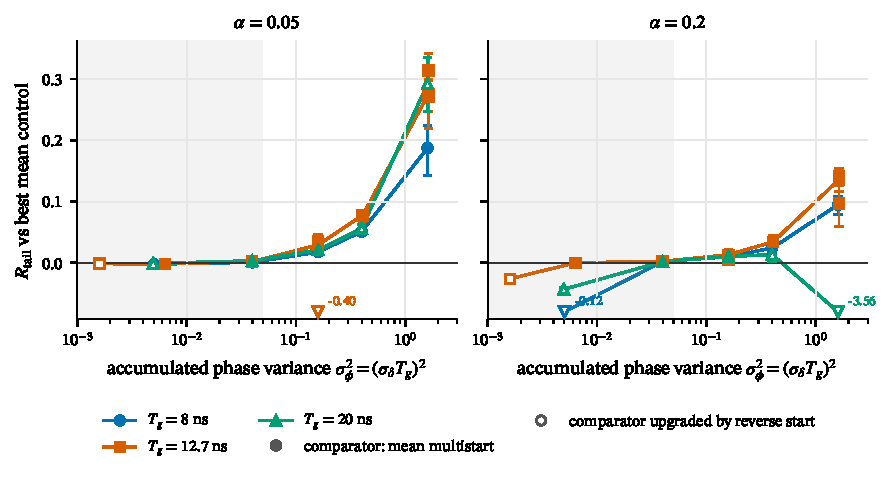
\includegraphics[width=0.84\textwidth]{fig_collapse.pdf}
\caption{The equivalence boundary. $\Rt$ versus accumulated phase variance
$\sigma_\phi^2=(\sigma_\delta T_g)^2$ at three gate times, two-level qubit,
detuning noise only, against the best mean control. Shaded:
$\sigma_\phi^2<0.05$, where the residual of Theorem~\ref{thm:main} is
negligible. Open markers: comparator upgraded by a reverse start; unconnected
points at $T_g=12.7$~ns are replication seeds; values below the axis are
marked at its lower edge (comparator asymmetry, \sref{sec:pitfalls}).}
\label{fig:collapse}
\end{figure*}

For $\sigma_\phi^2\le0.04$, $\Rt$ is zero within its confidence interval at
all three gate times: the numerical optimizers return controls with the same
tail, as the theorem requires. Beyond $\sigma_\phi^2\approx0.1$ the gain grows
smoothly and monotonically, to $0.19$--$0.29$ at $\sigma_\phi^2=1.6$. The
curves collapse: at $\sigma_\phi^2=0.16$ the three gate times give $0.018$,
$0.029$ and $0.021$, and at $0.41$ they give $0.051$, $0.077$ and $0.056$. A
2.5-fold change of gate time at fixed $\sigma_\phi$ thus leaves both the onset
and the size of the effect nearly unchanged, as the $\delta/\Omega$ argument
of Sec.~\ref{sec:fail} predicts; only the shortest gate falls somewhat lower
at the largest phase variance.

The divergence is reproducible and is not an optimization artefact. At
$\sigma_\phi^2=1.6$ three independent noise seeds give
$\Rt=0.275$, $0.271$ and $0.314$, and a second, independent set of runs with
eight restarts gives $0.274$, $0.276$ and $0.290$ (Sec.~\ref{sec:dominance}).
At every divergent point the reverse warm start returns to $\umean$: the two
optima lie in one basin, and CVaR shifts the solution within it rather than
selecting a different pulse family. The shift is small, a few percent in the
norm of the pulse envelopes (\sref{sec:pulses}).

\subsection{A direct test of the dominance premise}
\label{sec:dominance}

The comparison above tests a consequence of the theorem, namely that two
optimizers return the same control. The theorem states more: under
(A1)--(A2) the loss distributions of \emph{all} controls are rescaled copies
of one shape, so all pairs of controls are ranked identically by all risk
measures. We tested this directly over large pools of controls.

At each of 42 settings (two levels at $T_g=8$, $12.7$ and $20$~ns plus two
additional noise seeds at 12.7~ns; four levels at 12.7 and 20.8~ns; the six
phase variances above), the full comparison was repeated with eight restarts
per objective and every L-BFGS-B iterate of every run was recorded. A thinned
subset of iterates together with every final control forms a pool of
376--491 candidate controls, which we evaluated on a fresh ensemble of 4000
draws split into two independent halves. Over the \emph{competitive}
candidates (mean loss within a factor of two of the best) we computed: the
Kendall rank correlation $\tau$ between the orderings by mean and by
$\cvar_{0.05}$ (theorem: $\tau=1$); the fraction of \emph{confirmed rank
reversals}, among pairs separated by more than 2\% in both measures on both
halves, in which the two measures disagree with the same orientation on both
halves (theorem: 0); the fraction of pairs with at least 10\% difference in
mean whose quantile functions cross by more than 2\% in the upper half of the
distribution (theorem: 0); the ratio $\cvar_\alpha/\text{mean}$ of every
candidate (Proposition~\ref{prop:ratio}: $5.58$ and $3.25$); and a
cross-fitted \emph{pool regret} $R_{\mathrm{pool}}$, the CVaR gain of the
best-CVaR over the best-mean candidate when both are selected on one half and
scored on the other. The statistics were validated before the run on
synthetic families: an exactly ordered family $\sin^2(\sigma_iZ/2)$ gives
$\tau=1$ and no reversals, and the pre-compensation family $(Z^2-c_i)^2$ of
Remark~\ref{rem:precomp} gives $\tau=-0.46$ and 76\% reversals.

\begin{figure*}[t]
\centering
\includegraphics[width=0.9\textwidth]{fig_stage2_tests.pdf}
\caption{Direct test of the dominance premise over pools of 376--491
candidate controls per setting (closed markers: first noise seed; open: two
replication seeds). Shaded: $\sigma_\phi^2<0.05$. Dotted: the theorem's
prediction. (a) Kendall $\tau$ between the rankings by mean and by
$\cvar_{0.05}$. (b) Fraction of well-separated pairs whose rankings are
reversed, confirmed on two independent halves of a fresh 4000-draw ensemble.
(c) Fraction of pairs whose quantile functions cross in the upper half of the
distribution. (d) Cross-fitted pool regret against the full-Lindblad $\Rt$ of
the standard comparison (Spearman $0.90$, 42 settings); dashed: equality.}
\label{fig:dominance}
\end{figure*}

\begin{figure*}[t]
\centering
\includegraphics[width=0.9\textwidth]{fig_stage2_shape.pdf}
\caption{Shape test. (a) Median $\cvar_{0.05}/\text{mean}$ over the
competitive candidates (bars: interquartile range) versus $\sigma_\phi^2$.
Dotted: $5.58$ (Proposition~\ref{prop:ratio}). On the transmon the ratio is
lower at small noise because a noise-independent leakage floor makes up
56--84\% of the mean loss. (b) Complementary distributions of the loss divided
by the mean loss for 40 competitive candidates at $T_g=12.7$~ns. At
$\sigma_\phi^2=0.0016$ (blue) all collapse onto the $\chi^2_1$ shape (dashed);
at $\sigma_\phi^2=1.6$ (orange) they fan out and cross.}
\label{fig:shape}
\end{figure*}

On the two-level qubit the premise holds exactly where the theorem says it
should (Fig.~\ref{fig:dominance}). At $\sigma_\phi^2\le0.0064$ there is not
one confirmed rank reversal among 19\,639 well-separated pairs, over ten
settings, three gate times and three noise seeds. At $\sigma_\phi^2=0.04$
reversals stay below 0.8\%, and no pair crosses in the upper half of the
distribution at any two-level setting with $\sigma_\phi^2\le0.04$. The shape
prediction holds to 2\%: the median $\cvar_{0.05}/\text{mean}$ is
$5.49$--$5.60$ against $5.58$, and $\cvar_{0.2}/\text{mean}$ is
$3.23$--$3.24$ against $3.25$, with an interquartile spread below 1\% across
candidates. The normalized loss distributions of all competitive candidates
fall on the single $\chi^2_1$ curve [Fig.~\ref{fig:shape}(b)]. Even with a
free choice among hundreds of controls, CVaR has nothing to gain:
$R_{\mathrm{pool}}$ lies between $-0.002$ and $+0.001$. The rank correlation is
high but below one ($\tau=0.90$--$0.98$) because near-identical late
iterates are ordered by differences below the sampling noise; the
confirmed-reversal statistic, which requires a clear separation, is the
sharper test.

As $\sigma_\phi^2$ grows the premise fails, at the same threshold as the
optimized comparison. Reversals reach 10--13\% of pairs at
$\sigma_\phi^2=0.16$, 17--24\% at $0.41$ and 17--47\% at $1.6$; upper-half
crossings follow (3--5\%, 16--27\% and 27--68\%), and $\tau$ falls to
$0.10$--$0.62$. The onset is the same at all gate times and seeds. The shapes
stop collapsing: the lighter-tailed candidates carry more loss in the bulk,
the signature of pre-compensation (Sec.~\ref{sec:mechanism}). The pool regret
tracks the optimized-pair $\Rt$ (Spearman $0.90$, $p=4\times10^{-16}$), so
the optimized pair captures what the whole family of controls can offer.

One analysis choice needs stating. As first specified, the crossing test
compared entire quantile functions without a mean separation, and reported
4--31\% crossing pairs at $\sigma_\phi^2\le0.04$, where every other statistic
shows exact equivalence. All of these crossings lie
in the lower half of the distribution (median quantile $0.05$--$0.19$, none
above $0.46$), where a $\chi^2_1$ loss is tiny and is set by the residual
coherent error rather than by the noise; in 84--98\% of the crossing pairs the
control with the lower mean has the larger coherent error (29--78\% in one
seed). Theorem~\ref{thm:main} assumes no coherent error, and the mean and
CVaR are both governed by the upper half. We therefore restricted the test
to $q\ge0.5$ and to pairs that differ in mean, applied the restriction
uniformly, and report the unrestricted values in \sref{sec:crossing}.

\subsection{Leakage does not break the equivalence}
\label{sec:leakage}

The four-level transmon adds a physically distinct violation of (A2):
population transfer to levels $\ge2$ is a strongly nonlinear function of the
calibration errors. The nominal leakage of a Hann pulse of the correct area
falls from 3\% at 6.3~ns to the thermal floor ($6.8\times10^{-5}$) by about
20~ns, exceeding five times the floor below $T_g=12.7$~ns
(\sref{sec:leakonset}).

\begin{figure*}[t]
\centering
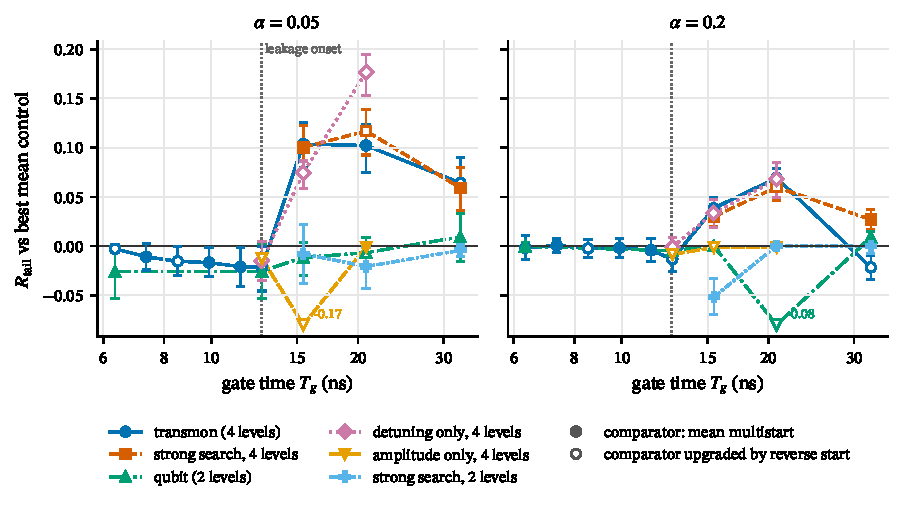
\includegraphics[width=0.84\textwidth]{fig_tg_sweep.pdf}
\caption{$\Rt$ versus gate time with detuning ($\sigma_\delta/2\pi=2.5$~MHz)
and amplitude ($\sigma_\gamma=2\%$) noise. Dotted: leakage onset. Open markers:
comparator upgraded by a reverse start; values below the axis are marked at
its lower edge. Throughout the leakage-dominated region the objectives
coincide. Above it, the transmon diverges and the two-level qubit with the
same noise does not, with 4 or 20 restarts; amplitude noise alone gives no
positive divergence.}
\label{fig:tg}
\end{figure*}

With both noise channels at their nominal widths
($\sigma_\delta/2\pi=2.5$~MHz, $\sigma_\gamma=2\%$), the mean and CVaR
controls coincide within $|\Rt|\le0.026$ throughout the leakage-dominated
region, $6.3\le T_g\le12.7$~ns, with four levels and with two
(Fig.~\ref{fig:tg}). Leakage is not absent from the problem; both
optimizers suppress it to $7$--$9\times10^{-5}$, and the residual loss
distributions remain ordered. Where $\Rt$ differs from zero at all it is
slightly negative, the out-of-sample penalty of estimating the tail from six
training draws.

Above the onset the transmon diverges and the qubit does not. With 20
restarts and 1000 iterations per objective, the transmon gives
$\Rt=0.100$, $0.117$ and $0.059$ at 15.4, 20.8 and 32.5~ns, while the
two-level qubit with identical noise gives $-0.008$, $-0.021$ and $-0.004$
($\sigma_\phi^2=0.06$, $0.11$ and $0.26$). Splitting the channels shows that
amplitude noise alone never produces a positive divergence; detuning noise
alone does (up to $0.18$ at 20.8~ns; \sref{sec:channelsplit}). This excludes
a mechanism in which the level-2 AC Stark shift converts amplitude error into
a quadratic phase. The higher levels therefore lower and amplify the
detuning-driven divergence, but on their own create none. The two-level
qubit with both channels shows no divergence at $\sigma_\phi^2=0.26$ and
$T_g=32.5$~ns, where the detuning-only scan would suggest a few percent; the
collapse of Sec.~\ref{sec:equiv} was tested only between 8 and 20~ns.

\subsection{Several channels at once}
\label{sec:channels}

Proposition~\ref{prop:twoaxis} allows two independent channels to separate
the objectives even at linear order. On the qubit at $T_g=12.7$~ns with
$\sigma_\delta/2\pi=2.5$~MHz we scanned the amplitude width up to
$\sigma_\gamma=12.7\%$ and the correlation $\rho$ between the channels
(\sref{sec:stage1}). With independent channels the objectives stay within a
few percent of each other; one point ($\sigma_\gamma=0.08$) is significant
and replicates only weakly ($+0.044$, $+0.028$, $+0.003$ over three seeds),
and the predicted geometric signature, a more isotropic loss for the CVaR
control, appears in one seed of three. The two-axis mechanism is real but
weak, because optimized controls can change the split of their error between
axes only slightly.

\begin{figure*}[t]
\centering
\includegraphics[width=\textwidth]{fig_lossdist.pdf}
\caption{Complementary cumulative distributions of the per-draw loss for the
mean control (blue) and the $\cvar_{0.05}$ control (orange), closed-system
model, 1000 test draws. Dotted: the worst 5\%. (a) Weak amplitude noise and
(b) strong independent channels: the distributions coincide, in the tail as
well as in the bulk. (c) Strongly correlated channels ($\rho=0.99$): they
\emph{cross}. The CVaR control is worse in the bulk (mean loss
$7.0\times10^{-4}$ against $4.4\times10^{-4}$) and better in the tail
($\cvar_{0.05}$ of $3.2\times10^{-3}$ against $4.6\times10^{-3}$).}
\label{fig:lossdist}
\end{figure*}

Correlating the channels, which reduces the noise to a single direction and
might be expected to restore equivalence, produces instead the largest
divergences in this scan: $\Rt=0.23$ at $\rho=-0.99$ and $0.29$ at
$\rho=+0.99$, with every reverse start returning to $\umean$. The loss
distributions cross [Fig.~\ref{fig:lossdist}(c)]. The reason is that
correlated noise lets the optimizer cancel one combined first-order error
direction instead of two, and it does: the linear response along the
dominant noise direction falls from $0.076$ at $\rho=0$ to
$0.013$--$0.017$ at $|\rho|=0.99$, and the mean loss of $\umean$ falls
fourfold. What remains is second order, with $\kappa$ above one. Rank-one
\emph{noise} is not rank-one \emph{linear error}: the optimization itself
removes the linearity on which equivalence rests. Correlation makes the
problem easier on average and harder in the tail.

\subsection{Mechanism: tail-targeted pre-compensation}
\label{sec:mechanism}

\begin{figure*}[t]
\centering
\panel{a}{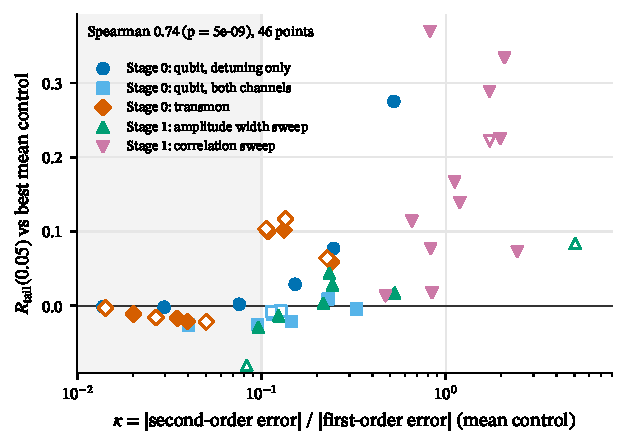
\includegraphics[height=4.6cm]{fig_kappa.pdf}}\hfill
\panel{b}{\includegraphics[height=4.6cm]{fig_stage2_kappa.pdf}}\hfill
\panel{c}{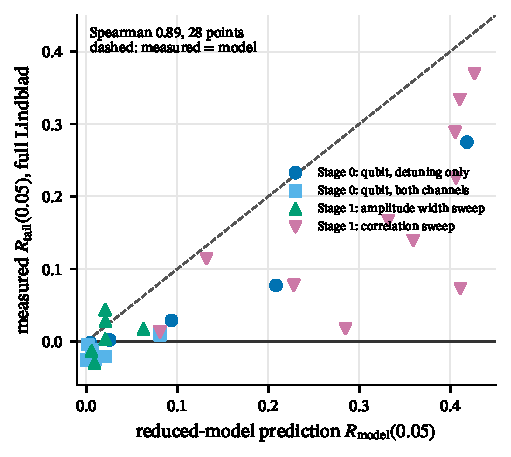
\includegraphics[height=4.6cm]{fig_model.pdf}}
\caption{One variable orders the divergence. (a) $\Rt(0.05)$ against the
second-order ratio $\kappa$ of the mean control, for every point with saved
error clouds (Spearman $0.74$, $p=5\times10^{-9}$, 46 points). (b) Fraction of
confirmed rank reversals in the candidate pools against $\kappa$ (Spearman
$0.87$, $p=4\times10^{-14}$, 42 settings); on the qubit reversals are absent
below $\kappa=0.076$ and present above $\kappa=0.13$. Shaded in (a,b):
$\kappa<0.1$. (c) Measured $\Rt(0.05)$ against the parameter-free prediction
$\Rm_{0.05}$ of Proposition~\ref{prop:reduced} for two-level points
(Spearman $0.89$, $p=1\times10^{-10}$, 28 points); dashed: equality. Open
markers: comparator upgraded by a reverse start.}
\label{fig:mechanism}
\end{figure*}

\paragraph*{$\kappa$ orders the results.} A single quantity, the
second-order ratio $\kappa$ of the mean control, orders the divergences of
all experiments [Fig.~\ref{fig:mechanism}(a)]. No point with
$\kappa\lesssim0.1$ shows a positive divergence. For a single channel $\kappa$
grows in proportion to $\sigma_\phi$ ($0.075$, $0.15$, $0.25$ and $0.5$ at
$\sigma_\phi^2=0.04$, $0.16$, $0.41$ and $1.6$), so $\kappa\approx0.1$
reproduces the threshold $\sigma_\phi^2\approx0.05$--$0.1$ of
Sec.~\ref{sec:equiv}. It also covers correlated channels, where the
cancellation of the linear error raises $\kappa$ at fixed noise strength. The
same threshold governs the whole control family: in the candidate pools, the
fraction of rank reversals is ordered by $\kappa$ and switches on between
$\kappa=0.076$ and $0.13$ [Fig.~\ref{fig:mechanism}(b)]. The transmon
diverges at somewhat smaller $\kappa$ (0.1--0.24), consistent with the
leakage contribution that $\kappa$ omits.

\begin{figure*}[t]
\centering
\includegraphics[width=\textwidth]{fig_kappa_bound.pdf}
\caption{The $\kappa^2$ law. (a) Reduced model with one dominant noise
direction: the relative tail gain against $\kappa$ (markers) and the
closed-form law $C_\alpha\kappa^2$ of Proposition~\ref{prop:kappa2} (lines),
with no fitted parameter. The gain saturates at the pre-compensation limit of
Remark~\ref{rem:precomp}. (b) The closed form against the numerically
optimized reduced model for every diagnosed control with $\kappa<0.35$; the
two agree over three decades (median ratio $1.07$, interquartile range
$0.94$--$1.12$ over 30 controls whose coefficients $C$ span $0.22$--$4.53$).
(c) Measured $\Rt(0.05)$ against $\kappa$, with the law for the two-level
detuning family ($C=4.5$) and the resolution of the study ($0.04$). Their
intersection, $\kappa=\sqrt{R_{\min}/C}=0.094$, falls between the largest
$\kappa$ at which no rank reversal is observed ($0.076$) and the smallest at
which reversals appear ($0.13$).}
\label{fig:kappabound}
\end{figure*}

\paragraph*{The gain is quadratic in $\kappa$, with the predicted
coefficient.} Proposition~\ref{prop:kappa2} makes the threshold quantitative,
and the saved error clouds test it directly. For each diagnosed mean control
we evaluated the closed form \eqref{eq:kappa2} from its fitted $A$ and $Q$ and
compared it with the numerically optimized reduced model
[Fig.~\ref{fig:kappabound}(b)]. Over the 30 controls with $\kappa<0.25$ the
ratio of prediction to model has median $1.07$ and interquartile range
$0.94$--$1.12$, although their coefficients $C$ differ by a factor of twenty
($0.22$ to $4.53$) and both one- and two-dimensional noise geometries are
present; the residual $7\%$ is the $O(\kappa)$ correction. The two-level
detuning family has $C=4.53$, nearly constant along the whole phase-variance
scan, so its gain crosses the resolution of this study at
$\kappa=\sqrt{0.04/4.53}=0.094$ [Fig.~\ref{fig:kappabound}(c)]. Measured:
no point with $\kappa\le0.10$ shows a significant divergence, and none of the
42 candidate pools with $\kappa\le0.076$ shows a rank reversal, while
reversals appear at every point with $\kappa\ge0.13$. The empirical threshold
of this paper is therefore a consequence of Theorem~\ref{thm:main}'s
hypothesis failing quadratically, not an independent finding.

One prediction is not confirmed. Equation~\eqref{eq:cstar} says the optimal
offset should fall from $4.15$ at small $\kappa$ to $2.76$ at large $\kappa$,
so the divergent points of the phase-variance scan ($\kappa\approx0.5$) should
sit near $3.4$. They sit at $2.46$--$2.54$, close to the $\kappa\to\infty$
value instead. The fixed-geometry model is the reason: a real optimizer also
reshapes $A$ and $Q$ rather than moving the offset alone, and it estimates the
tail from six training draws. The offset prediction is therefore quantitative
only in the limit, while the gain prediction \eqref{eq:kappa2} is accurate
where it is asymptotically valid.

\paragraph*{The reduced model predicts the size.} $\kappa$ is necessary but
not sufficient. At $\kappa\approx0.5$ detuning noise at
$\sigma_\phi^2=1.6$ gives $\Rt=0.275$, while independent channels at
$\sigma_\gamma=0.127$ give $0.017$. The difference is geometric: with one
dominant noise direction the second-order error of every tail draw points the
same way and one offset cancels it; with two independent directions it does
not. Proposition~\ref{prop:reduced} retains this geometry. Computed from each
mean control's fitted $A$ and $Q$ with no free parameter, $\Rm_{0.05}$
resolves the case above ($0.42$ against $0.06$--$0.08$) and orders the
measurements with Spearman correlation $0.89$ [Fig.~\ref{fig:mechanism}(c)],
against $0.83$ for $\kappa$ alone on the same points. It acts as an upper
envelope: measured values reach 6--87\% of it, and the two points above it
exceed it by less than their confidence intervals. The shortfall is expected,
since the Lindblad floor dilutes $\Rt$ and the real optimizer compares two
optimized controls rather than two offsets.

Once $\kappa$ is known, the experimental parameters add no further
information (\sref{sec:independence}). The correlation $|\rho|$ predicts
$\Rt$ on its own (Spearman $0.70$) but has partial correlation $-0.00$
($p=0.98$) given $\kappa$; the same holds for the noise strengths. Gate time
retains a borderline residual given $\kappa$ ($p=0.05$) that disappears given
$\Rm$ ($p=0.45$). Within these data, correlation, gate time and noise strength
act only through $\kappa$ and the error geometry, as
Proposition~\ref{prop:reduced} requires. The test is observational; the
parameters were not varied independently, and the controlled experiment of
Sec.~\ref{sec:controlled} shows that this conclusion is too strong for
$\kappa$ taken alone.

\begin{table}[b]
\caption{Prospective test at $\rho=0.99$, two levels: four points run after
the predictions were fixed. ``Fast'': closed-system value, without the
$T_1/T_2$ floor. $^{\circ}$Comparator upgraded by a reverse start.}
\label{tab:prospective}
\begin{ruledtabular}
\begin{tabular}{lcccc}
point & $\kappa$ & $\Rm_{0.05}$ & $\Rt(0.05)$ & fast\\
\hline
12.7~ns, noise $\times0.25$ & 0.84 & 0.285 & $0.018(8)$ & 0.156\\
12.7~ns, noise $\times0.5$ & 1.20 & 0.359 & $0.14(4)$ & 0.247\\
20~ns, matched $\sigma_\phi^2$ & 1.74 & 0.411 & $0.22(3)^{\circ}$ & 0.264\\
8~ns, matched $\sigma_\phi^2$ & 0.82 & 0.427 & $0.37(3)$ & 0.377\\
\hline
reference, 12.7~ns & 1.73 & 0.405 & $0.29(5)$ & 0.305\\
\end{tabular}
\end{ruledtabular}
\end{table}

\paragraph*{A prospective test.} To test the model on data it had not seen,
we fixed three predictions before running four new points
(Table~\ref{tab:prospective}): (a) $\Rt\le\Rm$ at every point; (b) $\Rt$
ranks as $\Rm$; (c) in the noise scan, $\kappa$ is proportional to the noise.
Predictions (a) and (b) hold at all four points, and the ranking is exact.
Prediction (c) fails ($\kappa\propto s^{0.5}$ over $s=0.25$--$1$). It
misapplied Proposition~\ref{prop:reduced}(ii), which holds for a
\emph{fixed} control: the mean control is re-optimized at each noise level
and cancels more of its linear error at lower noise, so $\kappa$ falls more
slowly than the noise. The 8~ns point gives the largest divergence of the
study, $\Rt=0.37$.

\begin{figure*}[t]
\centering
\includegraphics[width=0.62\textwidth]{fig_precomp_toy.pdf}\hfill
\panel{c}{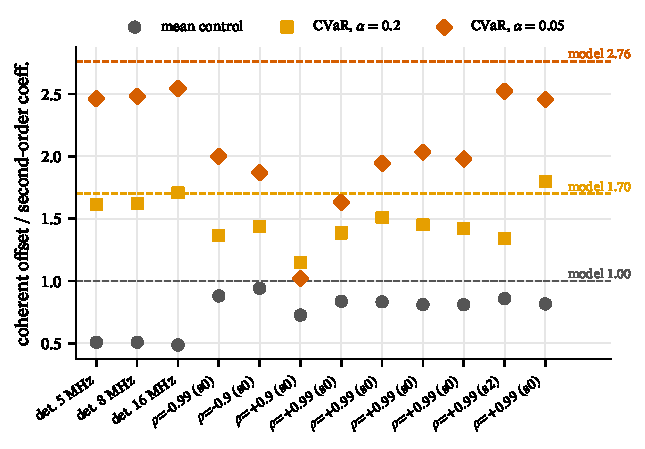
\includegraphics[width=0.36\textwidth]{fig_offset.pdf}}
\caption{Pre-compensation. (a) Per-draw loss $(z^2-c)^2$ of the
one-dimensional model of Remark~\ref{rem:precomp}; shaded: the worst 5\% of
draws. The mean optimum ($c=1$) cancels the error at $|z|=1$; the CVaR
optimum ($c=2.76$) cancels it at $|z|\approx1.66$ and accepts a large error at
$z=0$. (b) The resulting distributions cross near the 5\% level: the CVaR
choice has 2.5 times the mean loss but a 43\% lower $\cvar_{0.05}$.
(c) Measured coherent offset $c=-\mathbf e_0\cdot\mathbf q/|\mathbf q|^2$ of
the optimized controls at every significantly divergent point where one noise
direction dominates. Dashed: the parameter-free predictions $1$, $1.70$ and
$2.76$.}
\label{fig:precomp}
\end{figure*}

\paragraph*{What CVaR does.} The optimized controls behave as
Remark~\ref{rem:precomp} predicts [Fig.~\ref{fig:precomp}(c)]. At every
divergent point every CVaR control carries a coherent error antiparallel to
its second-order error (cosine $-1.00$). Across the phase-variance scan its
size is $2.46$--$2.54\,|\mathbf q|$ at $\alpha=0.05$ and
$1.61$--$1.71\,|\mathbf q|$ at $\alpha=0.2$, against $2.76$ and $1.70$
predicted. The mean controls sit near $c=1$ when their linear error is
cancelled ($0.73$--$0.94$ in the correlated-channel points) and near $0.5$
in the single-channel scan, where a large linear error remains. The shortfall at $\alpha=0.05$ is expected: the
optimizer can also reshape $A$ and $Q$, and it estimates the tail from six
draws. The same signature marks every divergent point: the nominal
(noise-free) loss is a much larger share of the mean loss for the CVaR
control than for $\umean$ ($0.83$ against $0.08$ at $\sigma_\phi^2=1.6$), while
in the equivalence region the two agree. CVaR does not find a lower-error
pulse. It trades nominal fidelity for a flatter tail, by pre-compensating the
second-order error of the worst draws.

\subsection{A controlled test of the mechanism variable}
\label{sec:controlled}

The evidence so far is observational: the experimental parameters were never
varied independently of $\kappa$. We therefore ran a designed experiment.
For each cell of a $3\times3$ grid in $(\rho,T_g)$ we \emph{solved} for the
noise scale that puts the mean control's $\kappa$ on a target value
$\kappa^\star\in\{0.20,0.35,0.55\}$, by secant iteration in $\log s$ over the
measured $\kappa(s)$ (\sref{sec:stage3design}), and then ran the standard
comparison there with two noise seeds: 27 cells, 54 points, all two-level.
Rows of the design differ in $\kappa$ and columns differ in the knobs at
approximately fixed $\kappa$.

\begin{figure*}[t]
\centering
\includegraphics[width=\textwidth]{fig_stage3_fixedkappa.pdf}
\caption{The controlled experiment at fixed $\kappa$. (a) $\Rt(0.05)$ against
the $\kappa$ of the control actually run; dotted lines mark the three target
values. The rows separate, but within each row the gate times do not overlap.
(b) The closed-form coefficient $C$ of Proposition~\ref{prop:kappa2} at each
target: at fixed $\kappa$ it spans three orders of magnitude, and the split is
by gate time. (c) Measured against the reduced-model prediction; the envelope
holds at 51 of 54 points.}
\label{fig:controlled}
\end{figure*}

\paragraph*{$\kappa$ orders the outcome.} Median $\Rt$ rises across the rows,
$+0.004$, $+0.037$, $+0.080$ (cells above the $T_1/T_2$ floor), and
$\mathrm{Spearman}(\kappa,\Rt)=+0.49$ over all 54 points.

\paragraph*{$\kappa$ does not explain it.} At fixed $\kappa$, gate time still
predicts the gain: the partial rank correlation of $\Rt$ with $T_g$ given
$\kappa$ is $-0.33$ ($p=0.015$), and $-0.58$ ($p<0.001$) among the cells whose
mean loss is above the dissipative floor. The claim of
Sec.~\ref{sec:mechanism}, that the knobs act on the divergence only through
$\kappa$, does not survive a controlled design; it was an artefact of how the
observational points happened to be distributed.

\paragraph*{The geometry is what is missing.} At fixed $\kappa$ the closed-form
coefficient $C$ of Proposition~\ref{prop:kappa2} varies by three orders of
magnitude, and it varies \emph{with gate time}: median $C=1.4$, $3.0$, $3.3$ at
$T_g=8$~ns for the three rows, against $0.02$--$0.09$ at $12.7$ and $20$~ns
[Fig.~\ref{fig:controlled}(b)]. A $\kappa$ of $0.35$ at 8~ns and a $\kappa$ of
$0.35$ at 20~ns are not the same physical situation: in the first the
second-order error is aligned with the dominant noise direction, in the second
it is not. Replacing $\kappa$ by the reduced model, which keeps that geometry,
removes the gate-time dependence entirely: the partial correlation of $\Rt$
with $T_g$ given $\Rm$ is $+0.01$ ($p=0.95$), and $-0.04$ ($p=0.84$) above the
floor, while $\mathrm{Spearman}(\Rm,\Rt)=+0.81$ there. The correlation
$\rho$ shows a residual effect given $\Rm$ over the full set ($-0.29$,
$p=0.03$) which disappears above the floor ($-0.12$, $p=0.49$): it comes from
the $\rho=0.9$ cells, whose mean losses of $\sim10^{-5}$ leave the CVaR
estimate dominated by its six training draws, and six of those eighteen cells
come out significantly \emph{negative}.

\paragraph*{Caveats of the design.} The calibration fixes $\kappa$ of the
control it optimizes, but the run's mean control is better optimized and
cancels more linear error, so its $\kappa$ is larger by a median factor
$1.08$ --- $1.30$ at 8~ns. The rows therefore overlap ($0.18$--$0.33$,
$0.35$--$0.56$, $0.51$--$0.74$) and every analysis above uses the measured
$\kappa$, not the target. The envelope property survives the design: three of
54 points sit above $\Rm$, none beyond its confidence interval.

\subsection{Leakage-aware $\kappa$}
\label{sec:leakage-kappa}

$\kappa$ is read from the qubit block of the error and is therefore blind to
leakage, which is why the transmon diverges at a smaller $\kappa$ than the
qubit. We extend the error coordinate to the leakage amplitudes,
$x=(\bm\epsilon;\,\mathrm{Re}\,l;\,\mathrm{Im}\,l)$ with
$l_{kj}=\langle k|U|j\rangle$ for $k\ge2$ in the same global-phase gauge, and
carry the loss metric with it: to second order
$L\approx x^{\mathsf T}Wx$ with $W=\mathrm{diag}(W_\epsilon,W_{\rm leak})$ and
$W_{\rm leak}=\tfrac{1+\lambda}{4}\big[\begin{smallmatrix}I\otimes G_r & -I\otimes G_i\\ I\otimes G_i & I\otimes G_r\end{smallmatrix}\big]$,
$G=\overline{\sum_\psi|\psi\rangle\langle\psi|}$ (\sref{sec:leakmetric}).
The mechanism variable becomes
$\kappa_{\rm lk}=\|W^{1/2}Q\|_F/\|W^{1/2}A\|_F$ in these coordinates.

\begin{figure*}[t]
\centering
\includegraphics[width=\textwidth]{fig_stage3_leakage.pdf}
\caption{Leakage-aware $\kappa$, over all 165 diagnosed mean controls (132
two-level, 33 four-level, 75 of them significantly divergent). (a) Divergence
threshold fitted separately for the two models; the factor between them falls
from $7.0$ to $1.7$. (b) $\Rt$ against $\kappa_{\rm lk}$, with the two
thresholds. (c) Leakage contributes a median $0.3\%$ of $\|A\|^2$ but $9.5\%$
of $\|Q\|^2$: it is almost entirely second-order error.}
\label{fig:leakkappa}
\end{figure*}

Re-diagnosing every saved control of every experiment with these coordinates
(no new optimization) gives three results. The decision thresholds of the two
models move together: fitted separately, the threshold is $0.387$ for the
qubit and $0.055$ for the transmon in $\kappa$, a factor of $7.0$, against
$0.248$ and $0.142$ in $\kappa_{\rm lk}$, a factor of $1.7$
[Fig.~\ref{fig:leakkappa}(a)]. The transmon is classified better
(AUC $0.949\to0.978$; pooled $0.732\to0.757$). And the leakage-aware reduced
model is an envelope for the transmon at 32 of 33 points, against 22 of 33 for
the qubit-only model. The reason is visible in the error budget: leakage is a
median $0.3\%$ of the first-order response but $9.5\%$ (up to $23\%$) of the
second-order term [Fig.~\ref{fig:leakkappa}(c)] --- exactly the quantity
$\kappa$ is meant to measure. The one remaining violation is the four-level
point at $T_g=20.8$~ns and $\sigma_\phi^2=0.41$, where $\Rt=+0.274$ against a
bound of $0.210$ with a confidence interval that excludes it.

\subsection{Generality: angle, anharmonicity and pulse basis}
\label{sec:generality}

Finally we varied the things the study had held fixed: the target rotation
angle ($\pi/4$, $\pi/2$, $\pi$), the anharmonicity ($-150$, $-200$,
$-300$~MHz, four levels) and the pulse basis (17 sine modes, 6 sine modes, and
17 piecewise-constant segments, the last matching the parameter count of the
first), each at two to four noise scales; 22 points
(\sref{sec:stage3generality}). Note that with an $x/y$ drive and no $z$
control a Hadamard is $X_{\pi/2}$ up to virtual-$Z$ frames, so the physically
distinct axis is the rotation angle, which sets the Rabi rate and hence
$\delta/\Omega$.

Over these points $\mathrm{Spearman}(\kappa,\Rt)=+0.82$ ($p=2\times10^{-5}$)
and $\mathrm{Spearman}(\Rm,\Rt)=+0.86$, with no detectable residual dependence
on anharmonicity ($p=0.24$) or basis ($p=0.84$). The anharmonicity scan is
the clean null: $\kappa=0.035$--$0.099$ across $-150$ to $-300$~MHz with
$\Rt$ between $-0.012$ and $+0.030$, every point inside its envelope. The
$\pi$ pulse behaves as the mechanism predicts and as spin echo would suggest:
it refocuses static detuning to first order, its linear response nearly
vanishes, $\kappa$ reaches $0.8$--$9.6$ and $\Rt$ reaches $0.28$--$0.55$ ---
but at mean losses of $10^{-8}$--$10^{-5}$, far below the $T_1/T_2$ floor,
so the effect is real in the closed system and invisible on hardware.

Two failures are worth recording. The piecewise-constant basis, at matched
parameter count, makes the optimization unreliable: at the nominal noise its
mean multistart misses a basin that the reverse start finds
($\Rt=-0.305$ against the recovered comparator), and at twice the noise it
exceeds its own envelope ($+0.132$ against $0.048$). This is a conditioning
failure of the search, not a property of the physics, and it means the
mechanism test is not portable to that basis without a better-conditioned
parameterization. Second, the raw comparison at these points was initially
misleading for a mundane reason: the closed-system $\Rt$ stored by the
pipeline is measured against the multistart mean control, and the
best-mean comparator of Sec.~\ref{sec:model} is applied by the Lindblad
validation step, which cannot run for a non-standard target. Applying the
comparator rule to the saved closed-system losses changed 46 of 76 Stage-3
points, by more than $0.05$ at four of them, and removed a spurious
$\Rt=+0.31$ at a setting where Sec.~\ref{sec:equiv} reports zero. It is the
same pitfall the protocol was built for, arriving through a new door.

\subsection{Colored noise: memory, and the effective dimension}
\label{sec:colored}

Every experiment so far has used quasi-static noise: one random draw held
fixed for the duration of the gate. Real dephasing has memory. Corollary
\ref{cor:general} says memory should change the size of $\sigma_\phi^2$ and
nothing else, which is a prediction the study had never tested. We replaced
the static detuning by an Ornstein--Uhlenbeck process of correlation time
$\tau_c$, sampled exactly as a stationary AR(1) sequence on the control grid
and normalized so that the accumulated phase variance
$\mathrm{Var}(\phi)=\sigma_{\mathrm{ou}}^2\,dt^2\sum_{jk}e^{-|t_j-t_k|/\tau_c}$
matches the quasi-static $\sigma_\phi^2$ at every $\tau_c$. That
normalization is what makes the comparison fair: the arms differ in the
\emph{shape} of the noise, not its integrated strength. The grid is
$\tau_c/T_g\in\{0.1,0.3,1,3,10\}$ plus a quasi-static arm, crossed with
$\sigma_\phi^2\in\{0.04,0.16,0.41\}$ and two seeds: $36$ points, all at
$T_g=12.7$~ns on the two-level model, with the best-mean comparator applied at
save time (it upgraded $20$ of the $36$, by at most $0.064$). Full protocol in
\sref{sec:stage4}.

\paragraph*{The control arm reproduces the static study.} The colored
propagator is a separate code path from the one used in
Secs.~\ref{sec:equiv}--\ref{sec:generality}, so its quasi-static limit is a
check on both. It gives $C=4.523$--$4.538$ across the six quasi-static points
against the $4.53$ of the detuning family in Sec.~\ref{sec:mechanism}, and
$\Rt=+0.028$ at $\sigma_\phi^2=0.16$ against the $+0.029$ of
Sec.~\ref{sec:equiv}.

\paragraph*{Memory does not move the comparison.} Across the whole grid
$|\Rt|\le0.043$, and the raw rank correlation of $\Rt$ with $\log\tau_c$ is
$+0.25$ ($p=0.14$), $+0.27$ controlling for $\sigma_\phi^2$ ($p=0.12$)
[Fig.~\ref{fig:stage4mem}(a)]. Corollary~\ref{cor:general} does not claim that
$\tau_c$ is invisible, however --- it claims that $\tau_c$ acts \emph{only} by
rescaling the effective noise, that is, only through $\kappa$ and the
geometry. The sharp test is therefore the one used in
Sec.~\ref{sec:controlled}: control for the reduced model as well. Doing so
removes the dependence entirely, to $+0.07$ given $\kappa$ ($p=0.70$),
$+0.10$ given $C\kappa^2$ ($p=0.59$) and $+0.05$ given $\Rm$ ($p=0.77$)
[Fig.~\ref{fig:stage4mem}(c)]. The same holds inside the only row where $\Rt$
is large enough to resolve: at $\sigma_\phi^2=0.41$, $\Rt$ does fall with
decreasing $\tau_c$ ($\mathrm{Spearman}=+0.65$, $p=0.02$), but it tracks
$C\kappa^2$ while doing so ($+0.67$, $p=0.02$), and the residual dependence on
$\tau_c$ given $C\kappa^2$ is $+0.21$ ($p=0.54$). Colored noise moves the
mechanism variable, and the mechanism variable moves the gain.

\paragraph*{What the pre-registered mechanism test can and cannot show.} The
two seeds put the run-to-run standard deviation of $\Rt$ at $0.021$ against a
total spread of $0.026$, so the reproducible signal has standard deviation
$0.015$ and \emph{any} correlation with $\Rt$ is attenuated by at most
$(1+\sigma^2_{\mathrm{noise}}/\sigma^2_{\mathrm{signal}})^{-1/2}=0.60$. The
pre-registered threshold for this stage was $0.6$, which therefore demanded a
perfect underlying correlation and could not be met. Against the ceiling, the
observed values are at it: $\mathrm{Pearson}(\Rm,\Rt)=0.67$, a regression
slope of $0.30\pm0.06$ --- properly inside $(0,1]$ for a bound --- and a
residual scatter of $0.019$, which is $0.93$ times the scatter between
repeats of the same cell [Fig.~\ref{fig:stage4mem}(b)]. The reduced model
leaves less unexplained variation than rerunning the experiment does. One
point of $36$ exceeds its $C\kappa^2$ envelope.

\paragraph*{Color raises the effective dimension.} The tail-to-mean ratio is
$5.36$ in the quasi-static arm, close to the $r_\alpha=5.58$ of
Proposition~\ref{prop:ratio}, and falls monotonically to $3.44$ at
$\tau_c=0.1\,T_g$, passing through the $4.00$ of
Proposition~\ref{prop:twoaxis} on the way. Read through
Proposition~\ref{prop:meff} this is not a failure of the shape prediction but
a measurement of $m_{\mathrm{eff}}$, which rises from $1.09$ to $2.8$
[Fig.~\ref{fig:stage4eff}(b)]. The mechanism is visible directly: a control
sees colored noise through more than the accumulated phase, and the share of
$\|A\|^2$ carried by the first-moment coordinate $z_2$ climbs from $0$ under
quasi-static noise to $0.70$--$0.84$ at short $\tau_c$
($\mathrm{Spearman}(\log\tau_c,\,z_2\text{ share})=-0.72$,
$p=8\times10^{-6}$).

The prediction can be made per control rather than per row. Taking the two
noise coordinates' shares of $\|A\|^2$ as the weights of
Eq.~\eqref{eq:meff} gives $\rho_\alpha(m_{\mathrm{eff}})$ from the control's
geometry alone, before any tail is examined. Where two coordinates actually
span the loss ($R^2_{\mathrm{fit}}\ge0.94$, $18$ points) the prediction
matches the measured ratio to a median of $2.6\%$, with
$\mathrm{Spearman}=+0.89$ ($p=8\times10^{-7}$)
[Fig.~\ref{fig:stage4eff}(a)]. Where they do not ($R^2_{\mathrm{fit}}$ as low
as $0.010$ at $\tau_c\le0.3\,T_g$), the measured $m_{\mathrm{eff}}$ exceeds
the two-coordinate participation ratio in $18$ of $18$ cases
($p=4\times10^{-6}$): the truncation fails, and it fails in the one direction
a truncation is allowed to fail. We regard that signed failure as better
evidence for Eq.~\eqref{eq:rhoeff} than uniform agreement would have been.

Two limitations follow. At $\tau_c\le0.3\,T_g$ the two-coordinate reduction
breaks down, so $C$ and $\Rm$ are not trustworthy there --- which is also
where $\Rt\approx0$, so little is at stake. And because the tail amplification
falls with $m_{\mathrm{eff}}$, fast noise is doubly unfavourable to a tail
objective: it lowers both the ratio that the objective exploits and, through
the fitted geometry, the coefficient $C$, which drops from $4.53$
quasi-static to $0.04$--$1.8$ at $\tau_c\le3\,T_g$. A device whose dephasing
is fast on the gate scale is a device where CVaR has least to offer.

\begin{figure*}[t]
\centering
\includegraphics[width=\textwidth]{fig_stage4_memory.pdf}
\caption{Colored noise. (a) $\Rt$ against the noise correlation time at three
phase variances, with the quasi-static limit at the right; lines are seed
means, faint markers the individual runs, and the band is the run-to-run
scatter. (b) $\Rt$ against the reduced-model prediction; the dotted line is
equality, the solid line the fit, and the band the replicate noise, which the
residual scatter already matches. (c) Partial rank correlation of $\Rt$ with
$\log\tau_c$ under successive controls: the dependence on correlation time
disappears once the mechanism variable is held fixed, as
Corollary~\ref{cor:general} requires.}
\label{fig:stage4mem}
\end{figure*}

\begin{figure*}[t]
\centering
\includegraphics[width=\textwidth]{fig_stage4_effdim.pdf}
\caption{The effective dimension. (a) Measured tail-to-mean ratio against the
participation ratio of the control's linear response; the curve is
$\rho_\alpha(m_{\mathrm{eff}})$ of Proposition~\ref{prop:meff} and the two
open circles are Propositions~\ref{prop:ratio} and~\ref{prop:twoaxis}. Points
for which two noise coordinates span the loss lie on the curve; points for
which they do not lie below it, because the truncation undercounts
directions. (b) $m_{\mathrm{eff}}$ inverted from the measured tail, against
correlation time. (c) The share of $\|A\|^2$ carried by the first-moment
noise coordinate, and the quality of the two-coordinate fit.}
\label{fig:stage4eff}
\end{figure*}

\subsection{The same curve along a second route}
\label{sec:geometry2}

Section~\ref{sec:colored} raised $m_{\mathrm{eff}}$ by giving the noise
memory. Nothing in Proposition~\ref{prop:meff} refers to memory, so the
sharper test is to raise $m_{\mathrm{eff}}$ by a mechanism with no time
structure at all and ask whether the ratio lands on the same curve. We did
that by rotating the noise between two physically distinct channels: a
detuning of variance $\sigma_\delta^2\cos^2\theta$ and a drive-amplitude
error of variance $\sigma_a^2\sin^2\theta$, with $\theta$ stepped in
$11.25^\circ$ increments from pure dephasing to pure amplitude noise and the
overall scale recalibrated at every $\theta$ to hold the mean loss fixed. Two
seeds, $T_g=12.7$~ns, two-level: $18$ points. Full protocol in
\sref{sec:stage1b}.

\paragraph*{The law holds, and the pre-registered statistic did not see it.}
Within a seed the agreement is close to exact: the measured ratio falls
monotonically as the participation ratio rises, with
$\mathrm{Spearman}(m_{\mathrm{eff}},\text{ratio})=-0.976$ and $-0.952$
against a predicted $-1$, and $\mathrm{Spearman}$ of prediction against
measurement of $+0.976$ ($p=3\times10^{-5}$) and $+0.952$
($p=3\times10^{-4}$), at median errors of $7.9\%$ and $3.4\%$
[Fig.~\ref{fig:stage5eff}(a)]. Pooled across seeds the same statistic is
$+0.712$, and the pre-registered threshold was $0.8$. The difference is a
nuisance level shift: seed~$1$ sits $+0.563\pm0.141$ above seed~$0$ in
measured ratio at every $\theta$, while the prediction varies by only $1.51$
over the whole range of $m_{\mathrm{eff}}$, so an offset of that size
reorders the pooled ranking without touching the law. Blocking on seed --- an
elementary precaution we should have pre-registered and did not --- gives a
seed-centred $\mathrm{Spearman}$ of $+0.962$ ($p=3\times10^{-9}$). We report
the pooled failure and the blocked pass together; the second is the
scientifically meaningful one and the first is a lesson about how to
pre-register.

\paragraph*{One curve, two mechanisms.} The two routes can now be compared
directly. Taking each point's residual from $\rho_\alpha(m_{\mathrm{eff}})$,
the colored-noise route gives a median of $-0.1\%$ with $10$th--$90$th
percentiles $[-7.4,\,+2.6]\%$ over $18$ points, and the channel-geometry route
a median of $-1.5\%$ with $[-8.0,\,+3.9]\%$ over $16$
[Fig.~\ref{fig:stage5eff}(b)]. A Mann--Whitney test does not distinguish them
($p=0.77$). Pooling all $34$ points against the single curve, with no
cross-calibration and no fitted constant, gives
$\mathrm{Spearman}=+0.831$ ($p=1\times10^{-9}$) at a median absolute residual
of $3.7\%$ [Fig.~\ref{fig:stage5eff}(c)], over closely matched coverage
($m_{\mathrm{eff}}\in[1.00,1.99]$ and $[1.00,1.92]$ respectively). Two
mechanisms with nothing physical in common --- one temporal, one
geometric --- put the tail-to-mean ratio on the same one-parameter curve.
That is the evidence that Proposition~\ref{prop:meff} describes a property of
the loss rather than of the experiment that suggested it.

\paragraph*{Two tests that did not resolve.} The design produced only one
pair separated by $\Delta m_{\mathrm{eff}}>0.3$, so the pre-registered
dominance-crossing test had no power and we do not score it. The pre-registered
$\kappa^2$-envelope test fails on $18$ points and passes on the $16$ in
regime: the two excluded points are at $\theta=90^\circ$, pure amplitude
noise, where the control nulls the linear response almost completely --- mean
losses of $5$--$6\times10^{-6}$ and $\kappa=6.3$ and $46.9$. A bound of the
form $R=C\kappa^2+O(\kappa^3)$ says nothing at $\kappa=47$. On the remaining
$16$, all with $\kappa\le0.12$, the largest exceedance is $0.027$ against a
threshold of $0.10$.

\subsection{Rare catastrophic channels: weight without leverage}
\label{sec:jumps}

Amplitude damping breaks (A1) in the way the theory is least equipped for: a
single trajectory either relaxes or does not, and the loss when it does is
set by the gate's structure rather than by a noise amplitude. We evaluated it
exactly rather than by trajectory sampling. Expanding the damped propagator
in the number of jumps and truncating after one gives a no-jump branch under
the Strang-split map $K_k=D^{1/2}U_kD^{1/2}$ and a one-jump branch whose
observable is accumulated by a single backward recursion, so the whole loss
distribution --- every branch, with exact weights --- costs one extra pass and
carries error $O((\Gamma T)^2)$. Two correctness subtleties are what make it
agree with the Lindblad channel: the branch probabilities differ per input
state, so the four-state average must be Bayes-weighted, and the jump weight
must be the telescoping trace loss of the discretized map rather than
$\Gamma\,dt\langle n\rangle$. With both, the residual mass defect over the
whole study is at most $2.2\times10^{-6}$. Derivation and validation in
\sref{sec:stage5}.

The grid crosses $T_g\in\{12.7,40\}$~ns, $T_1\in\{10,30\}\,\mu$s and
$\sigma_\phi^2\in\{0.04,0.16\}$ with two seeds, plus a four-level arm:
$14$ points, with $\beta$ spanning $0.098$ to $63$ and $p\le2.0\times10^{-3}$.

\paragraph*{The mixture law holds to one percent.} Across the twelve
two-level points the measured tail-to-mean ratio ranges from $8.20$ to
$19.87$ and Eq.~\eqref{eq:mixture} predicts it to a median of $1.2\%$, with
every point above $r_\alpha$ as required [Fig.~\ref{fig:stage5mix}(a)]. We
stress what is and is not being tested. The rank correlation between
prediction and measurement is $+0.991$, but the predicted ratio is a monotone
function of $\beta$ alone, so that number reproduces
$\mathrm{Spearman}(\beta,\text{ratio})$ to machine precision and is not an
independent check; the content of the test is the agreement in \emph{level},
at no free parameters, across a factor of $640$ in $\beta$. The four-level arm
is the one place the law degrades, to $9.9\%$ and $16.7\%$, in both cases with
the measurement below the prediction --- the signed direction expected when
leakage adds a third channel that a two-component mixture does not carry.

\paragraph*{And the optimizer ignores it.} A jump share of $63$ means the
rare branch supplies $98\%$ of the mean loss, and Eq.~\eqref{eq:xi} says a
tail objective weights it $3.58$ times more heavily still. Neither fact moves
the selected pulse. Over the $14$ points $|\Rt|\le0.13$ with a largest
positive value of $0.030$, and $\mathrm{Spearman}(\beta,\Rt)=+0.22$ ($p=0.45$)
[Fig.~\ref{fig:stage5mix}(c)]. That null survives every subset we tried: the
twelve two-level points ($+0.11$), dropping the two points with $\beta>10$
($+0.17$), and scoring against the raw mean comparator instead of the best one
($+0.01$). As in Sec.~\ref{sec:colored} the replicate noise caps what any such
correlation can be --- run-to-run standard deviation $0.032$ against a total
spread of $0.040$, a ceiling of $0.62$ --- so the honest reading is a
disattenuated $+0.36$, still far from significance. The companion prediction,
that $\kappa$ becomes inert once $\beta$ is present, does hold
($\mathrm{Spearman}(\kappa,\Rt)=+0.25$, $p=0.39$; partial given $\beta$,
$+0.18$, $p=0.56$), but a null on both variables is a weaker statement than
the substitution we predicted.

\paragraph*{Weight is not leverage.} The reason is visible in how little of
the jump channel the control can reach. Across the eight controls optimized
at each point --- free, mean, three tail levels and three reverse warm starts
--- the jump loss $\ell_j$ spans a median of $0.9\%$ and the integrated
excited population $n_{\mathrm{int}}$, which sets $p$, a median of $1.4\%$,
while the dephasing loss they are traded against spans $45\%$
[Fig.~\ref{fig:stage5mix}(b)]. The gate's own requirement pins the excited
population to within a percent, and the cost of a relaxation event is a
property of the target unitary, not of the pulse. A tail objective therefore
multiplies the weight on a channel whose shape the control cannot change,
and the extra weight has nowhere to act. This also explains why our
pre-registered estimator for the amplification failed: it scored the ratio
$(n_{\mathrm{free}}-n_{\cvar})/(n_{\mathrm{free}}-n_{\mathrm{mean}})$ against
$\Xi_\alpha=3.58$ and returned $0.72$, stable to $0.66$ as the resolution gate
is tightened from eleven points to five. That identity presumes
$n_{\mathrm{int}}$ is the coordinate along which the trade-off is resolved,
and the $1.4\%$-against-$45\%$ spread says it is not; the pulse moves almost
entirely in directions that leave $n_{\mathrm{int}}$ alone. The sign agrees at
$13$ of $14$ points and the magnitude means nothing, and we report the
estimator as mis-specified rather than the prediction as falsified.

\paragraph*{A pulse that nulls the linear response.} Two of the
$\sigma_\phi^2=0.16$ cells illustrate both halves at once. At one seed the
optimizer found a basin with the linear phase response almost entirely
cancelled: the dephasing loss drops by a factor of $73$ against its sibling
seed, the mean loss improves from $2.8\times10^{-3}$ to $1.4\times10^{-3}$,
and because $\|A\|_F$ collapses, $\kappa$ rises from $0.13$ to $6.2$ and
$\beta$ to $63$. Every one of the eight controls at that point lands in the
same basin, so it is a property of the problem and not of one restart. It is
the most tail-dominated pulse in the study by a wide margin --- and $\Rt$
there is $-0.0008$. When the remaining loss is carried by a channel the pulse
cannot shape, driving $\beta$ up does not create a tail-mean separation; it
only moves the ratio along Eq.~\eqref{eq:mixture}.

\paragraph*{What this adds to the scope.} Section~\ref{sec:mechanism}
established that the tail gain is quadratically small in $\kappa$. This
section adds a condition that $\kappa$ does not capture. A channel can
dominate the mean loss, sit far out in the tail, and be amplified several-fold
by the objective, and still not change the answer, because selection responds
to the \emph{gradient} of a channel with respect to the control and not to its
weight in the objective. A rare catastrophic channel is therefore not by
itself a reason to reach for a tail objective. The question to ask of a device
is not how heavy its worst channel is but how much of it the pulse can move.

\begin{figure*}[t]
\centering
\includegraphics[width=\textwidth]{fig_stage5_effdim_unified.pdf}
\caption{The effective dimension along a second route. (a) Measured
tail-to-mean ratio against the participation ratio as noise is rotated from
pure dephasing to pure amplitude error, shown separately by seed; the curve is
$\rho_\alpha(m_{\mathrm{eff}})$ of Proposition~\ref{prop:meff}. The two seeds
track the curve with a constant offset between them, which is what defeats a
pooled rank statistic. (b) Residuals from that curve for the colored-noise
route of Sec.~\ref{sec:colored} and the channel-geometry route here; ticks are
medians, bars the $10$th--$90$th percentiles. (c) All $34$ points against the
prediction, with no free parameter and no cross-calibration.}
\label{fig:stage5eff}
\end{figure*}

\begin{figure*}[t]
\centering
\includegraphics[width=\textwidth]{fig_stage5_mixture.pdf}
\caption{A rare catastrophic channel. (a) Measured tail-to-mean ratio against
the jump share $\beta$; the curve is Eq.~\eqref{eq:mixture} with no fitted
parameter, and the dotted lines are the two limits $r_\alpha$ and $1/\alpha$.
(b) How much of each quantity the control can reach: spread across the eight
controls optimized at a point, for the jump loss, the integrated excited
population that sets the jump probability, and the dephasing loss they are
traded against. The jump channel is nearly immovable. (c) The tail gain
against $\beta$, with the band showing the run-to-run scatter. Even at
$\beta=63$, where the rare branch carries $98\%$ of the mean loss, the two
objectives select the same pulse.}
\label{fig:stage5mix}
\end{figure*}

% =====================================================================
\subsection{Predicting the gain before paying for it}
\label{sec:predictor}

Everything so far diagnoses the gain after both optimizations have been run.
For the result to be useful on hardware the order has to be reversed: one
should be able to decide, from measurements on the mean-optimal pulse alone,
whether a tail objective is worth the shots. This section builds that
predictor and measures how well it works.

The construction is the reduced model of Proposition~\ref{prop:reduced} read
backwards. Let $\epsilon_k$ be the error coordinates of draw $k$ under the
mean-optimal control and $L_k=\epsilon_k^{\mathsf T}W\epsilon_k$ its loss. The
$\alpha$-tail selects a sub-population; its conditional mean displacement
\begin{equation}
d_\alpha \;=\; \E\!\left[\epsilon \,\middle|\, L \ge \mathrm{VaR}_\alpha(L)\right]
              \;-\; \E[\epsilon]
\label{eq:disp}
\end{equation}
is the direction in which the tail draws differ from the ensemble, and a
common offset $-t\,d_\alpha$ applied to every draw trades bulk loss for tail
loss. The optimal $t$ follows from a one-dimensional line search over the
measured losses, which requires no model of the control at all. Two
refinements matter in practice and are derived in the \SM: the
curvature of $\cvar_\alpha$ in the offset is not $2W$ but carries a boundary
term from draws entering and leaving the tail, and the step must be projected
onto the reachable subspace $\mathcal{B}=\operatorname{range}(\partial
\epsilon/\partial c)$. We write the resulting prediction $R_{\mathrm{pred}}$.
Every ingredient---$\epsilon_k$, $L_k$, $W$, and the Jacobian---is
measurable.

\emph{A protocol correction.} Scoring $R_{\mathrm{pred}}$ against a measured
gain requires a mean-side comparator, and our first attempt at a fair one was
wrong in a way worth recording. Following Sec.~\ref{sec:equiv} we scored the
CVaR control against the best of $\{\umean\}\cup\{\text{reverse warm
starts}\}$, a reverse warm start being a mean optimization initialized at a
CVaR solution. In $10$ of $16$ cells at least one reverse run found a
strictly \emph{better mean optimum} than the mean multistart itself, by a
factor of four in one cell. Where that happens the comparator is not a
fairness correction: the mean arm has effectively had five restarts, four of
them initialized with knowledge of where the good basins lie, against the
CVaR arm's one. The symptom was unmistakable in hindsight---the raw gain
$R^{\mathrm{raw}}$ was positive at $61$ of $64$ point--$\alpha$ pairs while
the comparator-based gain was negative at half of them.

The repair is symmetry. We pool every control any arm found at a point,
deduplicate, and run \emph{every} objective from \emph{every} start in that
pool, each arm reporting its best as selected on the validation ensemble by
its own risk measure, with the test ensemble touched only for the final
evaluation. Equal budget, equal information, and no arm selects on the
quantity being compared. The effect is large: the replicate scatter in $R$
between the two seeds fell by a factor of $10$ to $27$, from $0.272$ to
$0.010$ at $\alpha=0.2$ and from $0.178$ to $0.033$ at $\alpha=0.05$. All
numbers below use the pooled protocol. That almost all of the run-to-run
scatter in the earlier stages was optimizer basin selection rather than
anything physical is, we think, the single most useful practical lesson in
this work.

\emph{Direction.} The predicted displacement direction is essentially exact.
The cosine between the measured offset change $\Delta\epsilon_0$ and
$-d_\alpha$, taken in the $W$ metric, has median $0.997$, $0.999$, $0.980$
and $0.992$ at $\alpha=0.2$, $0.1$, $0.05$ and $0.025$, with Fisher-combined
null probabilities between $10^{-13}$ and $10^{-20}$ and not a single
significantly anti-aligned point. We restrict this statistic to points where
a local displacement model can apply at all---the gain must be resolved above
its own floor, the CVaR arm must not have found a better mean optimum (it
jumped basins rather than trading), and $|R^{\mathrm{raw}}|$ must exceed
$0.005$ so that there is a displacement to have a direction. All exclusions
and the ungated statistics are reported in the \SM. We note that a
minimum-cosine criterion, which we had pre-registered, is the wrong
statistic: $\cos=0.53$ in three dimensions has null probability $0.47$ and is
uninformative rather than contradictory.

\emph{Level.} Here the pre-registration failed and something better replaced
it. We had asked for a through-origin slope in $[0.7,1.3]$. The measured
slope is
\begin{equation}
s_\alpha \;=\; 0.588 \pm 0.025
\label{eq:calib}
\end{equation}
across the four $\alpha$ levels, and $0.589\pm0.033$ across all eight
$(\alpha,\text{seed})$ cells, with Spearman $\rho$ between $0.85$ and $0.97$
(Table~\ref{tab:stage6}, Fig.~\ref{fig:stage6cal}). Because scatter in the
dependent variable caps the attainable correlation rather than attenuating
the slope, the right comparison for $\rho$ is against that ceiling: the
ratios are $0.98$, $0.97$, $0.88$ and $0.98$. The predictor therefore
\emph{orders} the available gain almost perfectly and predicts its magnitude
up to one multiplicative constant, and that constant is flat in $\alpha$,
in $\kappa$ and in seed. Flatness in $\alpha$ is the informative part: a
finite-training-tail effect would scale with $\alpha$, since the CVaR
objective sees $64$ training draws at $\alpha=0.2$ and $8$ at $\alpha=0.025$,
and it does not.

The constant has a visible mechanism. The optimizer travels only part of the
predicted step: the ratio $\|\Delta\epsilon_0\|/\|t\,d_\alpha\|$ has median
$0.50$ (Fig.~\ref{fig:stage6cal}c). For a gain quadratic in the offset and
peaking at the predicted step, travelling a fraction $f$ returns $f(2-f)$ of
it, which is $0.75$ at $f=0.5$; the remainder is the geometry co-moving,
since the predictor holds $A$ and $Q$ fixed while the control moves. We do
not claim $0.588$ is universal. We claim it is a single constant on this
device family, measurable once, and that what a hardware experiment needs
from a predictor---which way to move and whether the move is worth
making---is the part that comes for free.

Two pre-registered tests remain untested rather than failed, and we say so
plainly. The resolution floor $R_{\min}$ sits at $\sim10^{-4}$ while every
point on our $\kappa$ grid predicts a gain above $3\times10^{-3}$, so the
below-floor null test (H4) never engaged; and the predicted boundary
$\kappa_c\approx0.0047$ lies below the smallest $\kappa$ we ran, $0.0253$, so
the observed boundary is a censoring bound and not a measurement. The
$\kappa^2$ law is at least self-consistent with it---at $\alpha=0.05$,
$C=4.53$ gives $R=1\times10^{-4}$ at $\kappa=0.0047$, which is the floor---but
that is arithmetic. Locating the boundary needs a predictor-only sweep down
to $\kappa\approx0.003$, which is cheap and which we did not run.

% =====================================================================
\subsection{What suppresses the gain: alignment, not rarity}
\label{sec:alignment}

Section~\ref{sec:jumps} found that a rare catastrophic channel adds weight to
the tail without adding leverage, and we generalized that to a claim about
rarity: any rare sub-population dominating the tail should suppress the gain,
because compensating it costs the overwhelming majority of ordinary draws.
That generalization is wrong, and the experiment built to confirm it refuted
it instead.

Define the bulk share of the tail loss,
\begin{equation}
\Lambda_\alpha \;=\;
\frac{\sum_{k\in\text{tail}\cap\text{bulk}} w_k L_k}
     {\sum_{k\in\text{tail}} w_k L_k},
\label{eq:leverage}
\end{equation}
which for the mixture of Proposition~\ref{prop:mixture} is
$\alpha\rho_\alpha/(\beta+\alpha\rho_\alpha)$ to first order in $p/\alpha$.
For the relaxation channel this is exactly the right quantity. Splicing the
recorded $(p,\beta)$ of each Stage~5 cell onto its measured dephasing
ensemble---the faithful reconstruction, since Stage~5 used the exact
no-jump/one-jump decomposition rather than sampling jumps---we find
$\Lambda_\alpha$ agreeing with the analytic bulk share to a median $0.24\%$,
and, more usefully,
\begin{equation}
\frac{R_{\mathrm{pred}}^{\mathrm{mix}}}{R_{\mathrm{pred}}^{\mathrm{bulk}}}
\;=\; \Lambda_\alpha
\label{eq:suppression}
\end{equation}
to a median $0.65\%$ and a worst case of $3.0\%$ over $40$ cell--$\alpha$
pairs spanning $\beta$ from $0.10$ to $3.3$ and $\Lambda$ from $0.70$ to
$0.075$ (Fig.~\ref{fig:stage6lev}a). Leverage does not merely correlate with
the gain; it multiplies it.

The counterexample is a two-state fluctuator: rare like a jump, but producing
a coherent phase error that the pulse can in principle reshape. Sweeping its
rarity $p$ at fixed excursion, with the fluctuator installed in the simulator
so that the optimizer, the losses and the propagators all see it, gives
Fig.~\ref{fig:stage6lev}b. Over a $25$-fold range in $p$, $\Lambda_{0.05}$
falls from $0.836$ to $0.018$---a factor of $46$---and
$R^{\mathrm{mix}}_{\mathrm{pred}}$ rises by $2.7$, while the \emph{measured}
gain does not move: $0.0167$, $0.0163$, $0.0154$, $0.0157$, flat to $4\%$.
Eq.~\eqref{eq:suppression} fails here by up to two orders of magnitude, and
fails in the direction of predicted enhancement.

The resolution is that $\Lambda_\alpha$ is a proxy, exact in one limit, for
the quantity that actually governs: the fraction of the tail loss the control
can reduce. A relaxation jump contributes a fixed loss that no pulse can
move, so its entire contribution is irreducible and the reducible fraction is
$\Lambda_\alpha$ exactly. A fluctuator that loads the same error coordinate
the bulk already loads is as reducible as the bulk is---the cosine between
the bulk-only and mixture offsets stays between $0.999$ and $0.944$ across
the sweep---so the reducible fraction stays near unity whatever $\Lambda$
does, and the gain is unchanged however rare the channel is. Consistently,
the measured gain tracks the \emph{bulk-only} predictor across the sweep, at
a ratio of $0.40$, $0.39$, $0.37$, $0.34$, while its ratio to the mixture
predictor falls from $0.37$ to $0.13$.

Both of our earlier readings named one axis of a two-axis quantity.
``Shapeable versus inert'' is the Stage~5 reading and is right about the
mechanism but silent about rarity; ``bulk versus rare'' is right about the
weights and silent about reducibility. What the two arms together establish
is that rarity alone does not suppress a tail gain, alignment does, and
Eq.~\eqref{eq:suppression} holds in the inert limit. An interpolation of the
form $\Lambda + (1-\Lambda)\cos^2$ reproduces the observed ratio drop across
the rarity sweep to about $6\%$; on four points we record that as a
conjecture and not a law.

For a hardware campaign this is the more useful statement of the two. The
question to ask of a noise channel is not how rare it is or how heavy its
worst realization is, but whether the correction it wants points the same way
as the correction the bulk wants---and that angle is estimable from
tail-conditional error coordinates, the same measurement the predictor of
Sec.~\ref{sec:predictor} already needs.

Two limits bound these claims. The rarity sweep leaves the mixture regime at
$p=0.1$, where $p/\alpha=2$ and the ``rare'' branch is twice the tail; and
the largest fluctuator excursions drive the two-coordinate fit quality to
$R^2=0.97$ and $0.68$, below which nothing computed from the reduced model is
interpretable. Separately, the fluctuator arm's measured gains were obtained
with a single multistart rather than the pooled protocol of
Sec.~\ref{sec:predictor}, so the flatness across the sweep, rather than any
individual value, is what carries the conclusion.

\begin{figure*}[t]
\centering
\includegraphics[width=\textwidth]{fig_stage6_calibration.pdf}
\caption{A measurement-only predictor of the tail gain. (a) Measured gain
against $R_{\mathrm{pred}}$ for the $16$ points of the $\kappa$ sweep at four
$\alpha$ levels; the solid line is the fitted through-origin slope
$0.588$ and the dashed line is the identity. (b) That slope against
$\alpha$, with single-seed values as ticks and the band showing
$\pm1$ standard deviation across $\alpha$; it is flat, which rules out a
finite-training-tail explanation. (c) The mechanism behind the constant: the
direction is predicted almost exactly (median $\cos>0.98$) while the
optimizer travels a median $0.50$ of the predicted step.}
\label{fig:stage6cal}
\end{figure*}

\begin{figure*}[t]
\centering
\includegraphics[width=\textwidth]{fig_stage6_leverage.pdf}
\caption{Alignment, not rarity, governs the suppression. (a) For the
control-inert relaxation channel, the ratio of the mixture prediction to the
bulk-only prediction equals the bulk share $\Lambda_\alpha$ of the tail loss
over two decades, with median error $0.65\%$ across $40$ cell--$\alpha$
pairs. (b) For a two-state fluctuator that loads the same coordinate as the
bulk, sweeping its rarity over $25\times$ moves $\Lambda$ by $46\times$ and
the mixture prediction by $2.7\times$ while the measured gain stays flat to
$4\%$ and tracks the bulk-only prediction instead. (c) Both arms on one axis:
$\Lambda$ is the inert limit of the reducible fraction, not a universal
suppression factor.}
\label{fig:stage6lev}
\end{figure*}

\begin{table}[t]
\caption{Calibration of the measurement-only predictor, by tail level.
Slopes are through the origin on $16$ points; the attenuation ceiling is the
largest correlation attainable given the replicate scatter in $R$, so
$\rho/$ceiling is the fraction of explainable variance the predictor
captures. The last row is the fraction of the predicted step the optimizer
actually travels.}
\label{tab:stage6}
\input{figures/tab_stage6.tex}
\end{table}

% =====================================================================
\section{Discussion}
\label{sec:discussion}

\paragraph*{What breaks the equivalence.} The theorem predicts the region in
which a tail objective is redundant, and its hypothesis (A2), measured as
$\kappa$, bounds that region. Of the four physical routes by which the
single-scalar structure can fail, leakage did not break it in our model;
both objectives suppress leakage to the thermal floor and the residual
distributions remain ordered. Two channels on different axes can break it
(Proposition~\ref{prop:twoaxis}), but only weakly in practice. Every large
divergence has one cause: second-order error that survives optimization,
which CVaR pre-compensates for the tail draws. It arises from large
accumulated detuning phase and, less obviously, from correlated channels,
whose cancellation of the linear error exposes the second-order term. The
fourth route, non-Gaussian randomness, we can now report on: trajectory-level
$T_1$ relaxation reshapes the loss distribution exactly as
Proposition~\ref{prop:mixture} says and yet does not change which pulse is
selected, for a reason that has no analogue in $\kappa$
(Sec.~\ref{sec:jumps}). Three further experiments sharpen this
picture: at fixed $\kappa$ the gate time still predicts the gain, so $\kappa$
orders the divergence without explaining it, while the geometry-aware reduced
model does explain it (Sec.~\ref{sec:controlled}); extending the error
coordinate to the leakage amplitudes brings qubit and transmon onto one
threshold (Sec.~\ref{sec:leakage-kappa}); and the mechanism survives changes
of rotation angle, anharmonicity and pulse basis (Sec.~\ref{sec:generality}).

\paragraph*{Deciding in advance, and what actually suppresses the gain.} Two
results change how the rest of this work would be used on a device. The
first is that the gain is predictable from measurements on the mean-optimal
pulse alone: the tail-conditional displacement gives the direction almost
exactly---median cosine above $0.98$ at every $\alpha$---and the magnitude up
to a single multiplicative constant $0.588\pm0.025$ that is flat in $\alpha$,
$\kappa$ and seed, with the predictor capturing $88$--$98\%$ of the
explainable variance in the measured gain (Sec.~\ref{sec:predictor}). One
decides whether to spend shots on a tail objective without first spending
them. The second corrects the reading we gave of the relaxation result. It is
not rarity that suppresses the gain but misalignment: the ratio of the
mixture prediction to the bulk-only prediction equals the bulk share of the
tail loss to $0.65\%$ for the control-inert jump channel, and fails by two
orders of magnitude for a fluctuator whose preferred correction points the
same way as the bulk's, whose rarity can be swept $25$-fold with no effect on
the measured gain at all (Sec.~\ref{sec:alignment}). The question to ask of a
noise channel is whether the pulse can move it, not how rare it is. A third
observation is methodological but was the largest single effect we measured:
most of the run-to-run scatter in these experiments was optimizer basin
selection, and equalizing the restart budget between the two objectives cut
the replicate scatter in the gain by a factor of $10$ to $27$.

\paragraph*{A test for practitioners.} The results reduce the decision
whether to use a tail objective to a measurement on the mean-optimal control.
(i) Optimize the mean as usual. (ii) Simulate $\umean$ on a few hundred noise
draws and extract the error rotation vectors. (iii) Fit
Eq.~\eqref{eq:expansion} and compute $\kappa$ and, preferably, $\Rm_\alpha$.
(iv) Compute the coefficient $C$ of Eq.~\eqref{eq:kappa2} from the same
fit and compare $C\kappa^2$ with the resolution $R_{\min}$ you can actually
measure. If $C\kappa^2\lesssim R_{\min}$ --- for one dominant noise direction
and $\alpha=0.05$, if $\kappa\lesssim0.32\sqrt{R_{\min}}$ --- stop: a tail
objective cannot improve the tail beyond estimation noise and can make it
slightly worse out of sample. Use $\kappa$ alone only as a screen: it is a
safe one, since no control with small $\kappa$ diverged anywhere in this study,
but it is not sufficient, because at fixed $\kappa$ the attainable gain still
varies by an order of magnitude with the error geometry that $C$ and $\Rm$
keep and $\kappa$ discards (Sec.~\ref{sec:controlled}). (v) Otherwise optimize CVaR warm-started from
$\umean$, with $\alpha K\gtrsim5$ training draws in the tail, and expect a gain
of at most $\Rm_\alpha$. For a single frequency-noise channel, step (iii) can be
replaced by the accumulated phase variance, known before any optimization:
below $\sigma_\phi^2\approx0.05$ CVaR is not worth running. With several
correlated channels $\kappa$ must be measured, because the optimizer itself
decides how much linear error remains. In our data the threshold
$\Rm_{0.05}>0.08$ classifies significant divergence correctly at 89\% of
points, and $\kappa>0.23$ at 82\%.

One diagnostic in this list costs nothing and needs no fit. The tail-to-mean
ratio of the mean-optimal control, already available from step (ii), gives
$m_{\mathrm{eff}}$ by inverting Eq.~\eqref{eq:rhoeff}. A ratio near $r_\alpha$
means a single noise direction reaches the gate, which is the regime the
closed-form coefficient of Table~\ref{tab:kappa2} describes; a ratio well
below it means several do, the tail is already lighter than the worst case,
and both the amplification a tail objective exploits and the fitted $C$ are
smaller (Sec.~\ref{sec:colored}). Dephasing that is fast on the gate scale is
the clearest instance. The same inversion works whatever raises
$m_{\mathrm{eff}}$: memory and channel geometry give residuals from
Eq.~\eqref{eq:rhoeff} that no test distinguishes (Sec.~\ref{sec:geometry2}).

\paragraph*{One caveat the screen does not cover.} Steps (iii)--(iv) measure
how nonlinear the residual error is. They do not measure how much of a channel
the control can actually move, and Sec.~\ref{sec:jumps} shows the two can come
apart completely: a relaxation channel carrying $98\%$ of the mean loss, sitting
above every other draw in the tail and weighted a further $3.58$ times by the
objective, produced no change in the selected pulse, because the gate
requirement pins its probability to within $1.4\%$ and its cost is fixed by the
target unitary. Where a heavy channel is suspected, the cheap follow-up is to
compare two controls that differ in mean loss and ask how much that channel's
contribution differs between them. If the answer is a percent, no reweighting
of it will change the answer, however far into the tail it sits.

\paragraph*{Relation to previous work.} Most robust-control methods target the
mean or a low-order expansion of the error: ensemble GRAPE and
sampling-based learning control average the fidelity over noise
\cite{Khaneja2005,Glaser2015,Chen2014}, sequential convex programming
bounds it \cite{Kosut2013}, and composite pulses, filter functions and
universally robust control cancel its leading-order sensitivities
\cite{Wimperis1994,Green2013,Poggi2024}. Our results state when these
approaches are already tail-optimal: whenever the residual error is linear
in Gaussian noise, a mean-optimal control is optimal for every monotone risk
measure. They also explain why cancelling the linear error, the aim of all
these methods, is what makes a tail objective matter, since it raises
$\kappa$. The exponential-utility controls of Ref.~\cite{Ge2021}, which
differed from average-fidelity controls, are covered by
Corollary~\ref{cor:general}, which gives a sufficient condition under which no
such difference is possible. On the risk side, the equivalence is an
instance of a general property of stochastic orders
\cite{Shaked2007,Follmer2016} and parallels the coincidence of mean--variance
and mean--CVaR portfolios for elliptical returns
\cite{Rockafellar2000,Embrechts2002}. What is specific to quantum gates is
the periodic loss, handled here with an explicit residual; the rotation
geometry, which breaks the ordering through majorization; and the
second-order structure of the error on a driven qubit, which breaks it
through pre-compensation.

\paragraph*{Physical reading.} A CVaR-optimized gate beyond the boundary is
deliberately miscalibrated. On a perfectly calibrated day it performs worse
than the mean-optimized gate, and it performs better on days with large
drift. Whether this is desirable depends on the error-correction layer: if
logical failure is dominated by the worst rounds, the tail is the relevant
quantity; if drifts are tracked and recalibrated frequently, the mean may be.
The present results show that the trade exists only at large $\kappa$ and can
be sized in advance from the mean control alone.

\paragraph*{Methodological note.} The comparison of two optimization
objectives is fragile. In the course of this work, seven distinct pipeline
errors produced publishable-looking but false conclusions, among them a
regularizer that manufactured $\Rt\approx0.3$ at the leakage onset, and a
comparator asymmetry that made CVaR look arbitrarily bad ($\Rt=-3.6$ in one
cell against $+0.11$ at equal search effort) (\sref{sec:pitfalls}). Search
effort is the central issue: a mean optimizer stuck in a poor basin makes any
alternative look good, and extra search on one side only makes the other look
bad. Neither the equal-budget nor the best-found comparison is safe alone. We
recommend the warm-start audit, the reverse warm start and the reporting of
both comparisons as standard practice for such studies.

\paragraph*{Limitations and outlook.} The noise is Gaussian, and $T_1$
enters only as a Lindblad channel: the one failure route of
Sec.~\ref{sec:fail} that the theorem cannot address is untested. The colored
study covers one gate time and the two-level model, and at
$\tau_c\le0.3\,T_g$ its two-coordinate reduction of the noise breaks down
($R^2$ as low as $0.010$), so $C$ and $\Rm$ are unreliable exactly where
$\Rt\approx0$; with two seeds per cell the reproducible spread of $\Rt$ there
is only $0.015$, which caps any rank correlation at $0.60$ and makes that
stage a test of consistency rather than of discrimination. Part (iv) of
Proposition~\ref{prop:meff} is numerical, not proved, and degrades as
$\alpha\to0$. The
reduced model optimizes only the offset, and its coefficient $C$ is read from
a least-squares fit of the error cloud, so it degrades where that fit does.
The controlled design fixes $\kappa$ of the control the calibration optimizes,
not of the one the run finally selects, which is larger by a median factor
$1.08$ and up to $1.74$, so its rows overlap; with two seeds per cell, a knob
effect below roughly a factor of two per cell would not be resolved. The
generality test covers the sine basis well and the piecewise-constant basis
poorly, because the latter optimizes unreliably at matched parameter count.
Natural next steps are trajectory-level $T_1$ statistics; non-Gaussian
noise, where assumption (A1) rather than (A2) is at stake; two-qubit gates, where the error geometry has more directions than the
offset can cancel; and a hardware test of the predicted crossing of the loss
distributions on a pulse-level superconducting processor.

% =====================================================================
\section{Conclusion}
\label{sec:conclusion}

When the gate error is linear in Gaussian noise, the error distributions of
all controls are rescaled copies of one shape, and the mean-optimal control is
optimal for CVaR and for every other law-invariant monotone risk measure. For
single-qubit gates under quasi-static detuning this holds while the
accumulated phase variance stays below about 0.05. There, over hundreds of
candidate controls per setting, the two objectives never disagree on a
well-separated pair, and every control shows the predicted tail-to-mean ratio.
Leakage does not change this. Beyond the boundary, the second-order error
of the mean-optimal control, measured by $\kappa$, decides whether and by how
much a tail objective helps: the attainable gain is quadratic in $\kappa$ with
a coefficient we give in closed form, so the threshold below which a tail
objective is redundant follows from the theory rather than from the data, and
a parameter-free reduced model predicts the size of the gain above it. What the tail objective then finds is a deliberately
miscalibrated gate that pre-compensates the second-order error of the worst
noise draws. A controlled experiment at fixed $\kappa$ shows that this scalar
orders the divergence but does not by itself explain it: the error geometry
that the reduced model keeps is what makes a gate at one duration different
from a gate at another with the same $\kappa$. Giving the noise memory does
not change any of this --- across two decades of correlation time the
comparison depends on the correlation only through that same coefficient ---
but it does change the shape of the tail, by spreading the error over more
noise directions. The tail-to-mean ratio measures how many, along a curve
that contains the single-channel and two-channel ratios as its first two
points --- and rotating the noise between two channels, a mechanism with no
time structure at all, puts the ratio on that same curve within the scatter of
the first route. A rare catastrophic channel is the one case where the shape of
the tail and the choice of pulse come apart. Adding $T_1$ relaxation at the
trajectory level moves the tail-to-mean ratio from 5.6 to almost the ceiling
$1/\alpha$, in quantitative agreement with a closed form, while leaving the
selected pulse untouched: the gate requirement fixes both the probability of
relaxation and its cost to within about a percent, so an objective that weights
that channel more heavily has nothing to act on. Selection responds to how much
of a channel the control can move, not to how much of the loss it carries.
A fluctuator sharpens the point: it is rare like a jump but loads the same
error coordinate the bulk does, and sweeping its rarity over a factor of
twenty-five changes the measured gain by four percent while the bulk share of
the tail moves by a factor of forty-six. What suppresses a tail gain is
misalignment between the correction the rare channel wants and the one the
bulk wants, and the bulk share is an exact proxy for it only in the inert
limit that relaxation happens to occupy.

Finally, none of this has to be discovered by running both optimizations. The
tail-conditional displacement of the error coordinates under the mean-optimal
control predicts which way a tail objective would move the gate---median
cosine above $0.98$---and how much it would gain, up to one multiplicative
constant near $0.59$ that is flat in the tail level, in $\kappa$ and in seed.
Since the displacement, the metric and the reachable subspace are all
measurable on hardware, the decision of whether a tail objective is worth its
shots can be made before any of them are spent. Robust gates can therefore be
designed for the mean, and tested for $\kappa$, for that alignment, and for
the predicted gain, before a tail objective is worth its cost.

\begin{acknowledgments}
The author thanks Dr.\ Boxi Li (RIKEN) for guidance and discussions.
\end{acknowledgments}

\paragraph*{Data availability.} The code and the data underlying the figures
are available from the author upon reasonable request.

% =====================================================================
\begin{thebibliography}{99}
\bibitem{Paladino2014} E.~Paladino, Y.~M.~Galperin, G.~Falci, and B.~L.~Altshuler, $1/f$ noise: Implications for solid-state quantum information, \href{https://doi.org/10.1103/RevModPhys.86.361}{Rev.\ Mod.\ Phys.\ \textbf{86}, 361 (2014)}.
\bibitem{Krantz2019} P.~Krantz, M.~Kjaergaard, F.~Yan, T.~P.~Orlando, S.~Gustavsson, and W.~D.~Oliver, A quantum engineer's guide to superconducting qubits, \href{https://doi.org/10.1063/1.5089550}{Appl.\ Phys.\ Rev.\ \textbf{6}, 021318 (2019)}.
\bibitem{Kjaergaard2020} M.~Kjaergaard, M.~E.~Schwartz, J.~Braum\"uller, P.~Krantz, J.~I.-J.~Wang, S.~Gustavsson, and W.~D.~Oliver, Superconducting qubits: Current state of play, \href{https://doi.org/10.1146/annurev-conmatphys-031119-050605}{Annu.\ Rev.\ Condens.\ Matter Phys.\ \textbf{11}, 369 (2020)}.
\bibitem{Khaneja2005} N.~Khaneja, T.~Reiss, C.~Kehlet, T.~Schulte-Herbr\"uggen, and S.~J.~Glaser, Optimal control of coupled spin dynamics: Design of NMR pulse sequences by gradient ascent algorithms, \href{https://doi.org/10.1016/j.jmr.2004.11.004}{J.\ Magn.\ Reson.\ \textbf{172}, 296 (2005)}.
\bibitem{Glaser2015} S.~J.~Glaser \emph{et al.}, Training Schr\"odinger's cat: Quantum optimal control, \href{https://doi.org/10.1140/epjd/e2015-60464-1}{Eur.\ Phys.\ J.\ D \textbf{69}, 279 (2015)}.
\bibitem{Chen2014} C.~Chen, D.~Dong, R.~Long, I.~R.~Petersen, and H.~A.~Rabitz, Sampling-based learning control of inhomogeneous quantum ensembles, \href{https://doi.org/10.1103/PhysRevA.89.023402}{Phys.\ Rev.\ A \textbf{89}, 023402 (2014)}.
\bibitem{Kosut2013} R.~L.~Kosut, M.~D.~Grace, and C.~Brif, Robust control of quantum gates via sequential convex programming, \href{https://doi.org/10.1103/PhysRevA.88.052326}{Phys.\ Rev.\ A \textbf{88}, 052326 (2013)}.
\bibitem{Weidner2025} C.~A.~Weidner, E.~A.~Reed, J.~Monroe, B.~Sheller, S.~O'Neil, E.~Maas, E.~A.~Jonckheere, F.~C.~Langbein, and S.~Schirmer, Robust quantum control in closed and open systems: Theory and practice, \href{https://doi.org/10.1016/j.automatica.2024.111987}{Automatica \textbf{172}, 111987 (2025)}.
\bibitem{Wimperis1994} S.~Wimperis, Broadband, narrowband, and passband composite pulses for use in advanced NMR experiments, \href{https://doi.org/10.1006/jmra.1994.1159}{J.\ Magn.\ Reson.\ A \textbf{109}, 221 (1994)}.
\bibitem{Green2013} T.~J.~Green, J.~Sastrawan, H.~Uys, and M.~J.~Biercuk, Arbitrary quantum control of qubits in the presence of universal noise, \href{https://doi.org/10.1088/1367-2630/15/9/095004}{New J.\ Phys.\ \textbf{15}, 095004 (2013)}.
\bibitem{Poggi2024} P.~M.~Poggi, G.~De~Chiara, S.~Campbell, and A.~Kiely, Universally robust quantum control, \href{https://doi.org/10.1103/PhysRevLett.132.193801}{Phys.\ Rev.\ Lett.\ \textbf{132}, 193801 (2024)}.
\bibitem{Ball2021} H.~Ball \emph{et al.}, Software tools for quantum control: Improving quantum computer performance through noise and error suppression, \href{https://doi.org/10.1088/2058-9565/abdca6}{Quantum Sci.\ Technol.\ \textbf{6}, 044011 (2021)}.
\bibitem{Fowler2012} A.~G.~Fowler, M.~Mariantoni, J.~M.~Martinis, and A.~N.~Cleland, Surface codes: Towards practical large-scale quantum computation, \href{https://doi.org/10.1103/PhysRevA.86.032324}{Phys.\ Rev.\ A \textbf{86}, 032324 (2012)}.
\bibitem{Rockafellar2000} R.~T.~Rockafellar and S.~Uryasev, Optimization of conditional value-at-risk, J.\ Risk \textbf{2}(3), 21 (2000).
\bibitem{Acerbi2002} C.~Acerbi and D.~Tasche, On the coherence of expected shortfall, \href{https://doi.org/10.1016/S0378-4266(02)00283-2}{J.\ Bank.\ Finance \textbf{26}, 1487 (2002)}.
\bibitem{Artzner1999} P.~Artzner, F.~Delbaen, J.-M.~Eber, and D.~Heath, Coherent measures of risk, \href{https://doi.org/10.1111/1467-9965.00068}{Math.\ Finance \textbf{9}, 203 (1999)}.
\bibitem{Barkoutsos2020} P.~Kl.~Barkoutsos, G.~Nannicini, A.~Robert, I.~Tavernelli, and S.~Woerner, Improving variational quantum optimization using CVaR, \href{https://doi.org/10.22331/q-2020-04-20-256}{Quantum \textbf{4}, 256 (2020)}.
\bibitem{Woerner2019} S.~Woerner and D.~J.~Egger, Quantum risk analysis, \href{https://doi.org/10.1038/s41534-019-0130-6}{npj Quantum Inf.\ \textbf{5}, 15 (2019)}.
\bibitem{Ge2021} X.~Ge and R.-B.~Wu, Risk-sensitive optimization for robust quantum controls, \href{https://doi.org/10.1103/PhysRevA.104.012422}{Phys.\ Rev.\ A \textbf{104}, 012422 (2021)}.
\bibitem{Embrechts2002} P.~Embrechts, A.~J.~McNeil, and D.~Straumann, Correlation and dependence in risk management: Properties and pitfalls, in \emph{Risk Management: Value at Risk and Beyond}, edited by M.~A.~H.~Dempster (Cambridge University Press, Cambridge, 2002), pp.~176--223.
\bibitem{Nielsen2002} M.~A.~Nielsen, A simple formula for the average gate fidelity of a quantum dynamical operation, \href{https://doi.org/10.1016/S0375-9601(02)01272-0}{Phys.\ Lett.\ A \textbf{303}, 249 (2002)}.
\bibitem{Shaked2007} M.~Shaked and J.~G.~Shanthikumar, \emph{Stochastic Orders} (Springer, New York, 2007).
\bibitem{Follmer2016} H.~F\"ollmer and A.~Schied, \emph{Stochastic Finance: An Introduction in Discrete Time}, 4th ed.\ (de Gruyter, Berlin, 2016).
\bibitem{Marshall2011} A.~W.~Marshall, I.~Olkin, and B.~C.~Arnold, \emph{Inequalities: Theory of Majorization and Its Applications}, 2nd ed.\ (Springer, New York, 2011).
\bibitem{Koch2007} J.~Koch, T.~M.~Yu, J.~Gambetta, A.~A.~Houck, D.~I.~Schuster, J.~Majer, A.~Blais, M.~H.~Devoret, S.~M.~Girvin, and R.~J.~Schoelkopf, Charge-insensitive qubit design derived from the Cooper pair box, \href{https://doi.org/10.1103/PhysRevA.76.042319}{Phys.\ Rev.\ A \textbf{76}, 042319 (2007)}.
\bibitem{Lindblad1976} G.~Lindblad, On the generators of quantum dynamical semigroups, \href{https://doi.org/10.1007/BF01608499}{Commun.\ Math.\ Phys.\ \textbf{48}, 119 (1976)}.
\bibitem{Byrd1995} R.~H.~Byrd, P.~Lu, J.~Nocedal, and C.~Zhu, A limited memory algorithm for bound constrained optimization, \href{https://doi.org/10.1137/0916069}{SIAM J.\ Sci.\ Comput.\ \textbf{16}, 1190 (1995)}.
\bibitem{Higham2008} N.~J.~Higham, \emph{Functions of Matrices: Theory and Computation} (SIAM, Philadelphia, 2008).
\bibitem{Efron1993} B.~Efron and R.~J.~Tibshirani, \emph{An Introduction to the Bootstrap} (Chapman \& Hall, New York, 1993).
\bibitem{SM} See Supplemental Material for full proofs, the model and simulator details, the fairness protocol and the pipeline errors it removed, simulator validation, additional results and per-point tables, and reproducibility information, which includes Refs.~\cite{VanLoan1978,Motzoi2009}.
\bibitem{VanLoan1978} C.~F.~Van~Loan, Computing integrals involving the matrix exponential, \href{https://doi.org/10.1109/TAC.1978.1101743}{IEEE Trans.\ Autom.\ Control \textbf{23}, 395 (1978)}.
\bibitem{Motzoi2009} F.~Motzoi, J.~M.~Gambetta, P.~Rebentrost, and F.~K.~Wilhelm, Simple pulses for elimination of leakage in weakly nonlinear qubits, \href{https://doi.org/10.1103/PhysRevLett.103.110501}{Phys.\ Rev.\ Lett.\ \textbf{103}, 110501 (2009)}.
\end{thebibliography}

\end{document}
